\documentclass[30pt,a4paper]{article}
% Dokumenten Typ, titelseite, Schriftgröße, Seitenformat
\PassOptionsToPackage{dvipsnames}{xcolor}
% Füge neue Farben hinzu (standart 5 farben oder so)
\usepackage[utf8]{inputenc}
% Kodierung
\usepackage[T1]{fontenc}
% Umlaute
\usepackage[german]{babel}
% Eingebundene Sprachen
\usepackage{graphicx}
% Einbinden von Grafiken
\usepackage{wrapfig}
% Text um kleine Grafiken herumsetzen
\usepackage{amsmath}
\usepackage{amsfonts}
\usepackage{amssymb}
% Mathe Symbole und Commands
\usepackage{mathtools}
% Verbessert ams Packete von oben
\usepackage{nicefrac}
% Schönere Brüche
\usepackage{tikz}
\usepackage{circuitikz}
\usepackage{tikz-cd}
% Tikz Stuff
\usepackage{enumerate}
% Bessere Aufzählungen
\usepackage{cancel}
% z.B Durchstreichen von Sachen
\usepackage[hidelinks]{hyperref}
\usepackage{cleveref}
% Links und Referenzen innerhalb des Dokuments
\usepackage{tcolorbox}
% Wunderschöne Farbige Boxen mit Überschriften
\usepackage{caption}
% Erstellen von captions innerhalb einer Minipage
\usepackage[margin=1in]{geometry}
% Änderung der Gestaltung einer Seite (Überschreibt \documentclass)
\usepackage{placeins}
% Mit Hilfe von \FloatBarrier floats einschränken
\usepackage{booktabs}
% Bei Tabellen wird kann anstelle von \hline \toprule, \midrule und \bottomrule verwendet werden etc.
\usepackage{wasysym}
% Fügt eine Reihe von Symbolen wie Männlich Weiblich dazu
\usepackage{url}
% Füge Problemlos urls ein
\usepackage{pdfpages}




\hbadness=99999 
% Löst ein Problem mit \hbox

\newenvironment{Dtabular}[2][1] {\def\arraystretch{#1}\tabular{#2}}
{\endtabular}

\title{
	\large Fortgeschrittenes Physik Lab	SS19 \\[4mm]
	\textbf{\LARGE Experiment: Szintillationszähler
	} \\[4mm]
	(Durchgeführt am: (07.-08).10.19 bei Patrick Scholer) \\}
% Titel des Experiments
\author{Erik Bode, Damian Lanzenstiel \\ (Group 103)}
% Autoren

\begin{document}
	
	\begin{titlepage}
		\maketitle
		\vspace{2cm}
		\begin{abstract}
			Während dieses Versuches wurden mehre NIM-Module in Funktionsweise und Signalform betrachtet. Anschließend sind Spektren von $^{22}Na$, $^{60}Co$, $^{152}Eu$ und $^{228}Th$ aufgenommen worden. Bei den ersten drei Isotopen gelang die Identifikation der erwarteten gemessenen Energien gut, bei Thorium stellte sich dies herausfordernder dar. Anschließend wurde die Winkelabhängigkeit der Vernichtungsphotonen ausgelöst durch Paarbildung gemessen.
		\end{abstract}
	\end{titlepage}
	\newpage
	\tableofcontents
	\listoftables
	\listoffigures
	\newpage
	\section{Theory}
The contents of this chapter are, if not otherwise specified, derived from the guide to the experiment \cite{anleitung}
\subsection{Spin and nuclear spin}
The spin or intrinsic angular momentum of a elementary particle is an intrinsic property of particles from the family of the fermions. Members of this family, such as protons, neutrons and electrons all have a spin of $s=\frac{1}{2}$.
The spin can be explained semi classically, as rotation of the particle around its own 'centre of mass', with fixed frequency and variable axis of rotation. 
However, this illustration only makes sense in finite-size particles, of course. Just as with the angular momentum, not all three spin components can be defined at the same time, but only the amount and projection on a freely selectable 'quantization axis'.
The possible spin quantum numbers are $$ \left|\vec{S}\right| = \hbar \sqrt{S\left(S+1\right)}$$ with $S = 0, \frac{1}{2}, 1, ...$ and Planck's constant $\hbar$. 
Atomic nuclei are also assigned a spin, the nuclear spin, which is defined with the nuclear spin number $I$, analogue to the spin: 
$$\left|\vec{I}\right| = \hbar \sqrt{I\left(I+1\right)}$$
The nuclear spin number is also quantified in its direction. Analogue to the electron spin, the projection of the nuclear spin can also assume certain states as , e.g. with the z-axis as the quantization axis $I_z = m_I \hbar$ with $-I\le m_I \le + I$. In total there would be  $2I+1$ different states for $I_z$. Protons or the nucleus of $^{19}$F both have a nuclear spin number of $I=\frac{1}{2}$. So both have only two possible states: $m_I = \pm \frac{1}{2}$. They can only align parallel or antiparallel with the quantization axis in the experiment.

\subsection{Magnetic momentum}
The spin of a quantum mechanical particle is connected to a magnetic dipole momentum $\vec{\mu}$, the ratio of both is described as the gyromagnetic ratio $\gamma$.
$$\vec{\mu}=\gamma\vec{I}\qquad \textrm{with}\quad \gamma = \frac{g_I\mu_K}{\hbar}$$
The constant $g_I$ is the nuclear g factor, which is to be calculated during the exam. $g_I$ has no dimension and is unique for each nucleus. The second constant $\mu_K$ is the nuclear magneton, which is computed analogue to the Bohr magneton:
$$\mu_K = \frac{e\hbar}{2m_p}$$
The difference between those two is that for the Bohr magneton the elecron mass is used and for the nuclear magneton the proton mass. 
In the ground state of atomic nuclei, the nucleons are arranged according to the Pauli principle so that each orbital is occupied by two protons or neutrons of opposite spins. If now a eu-nucleus (with an even number of protons and an uneven number of neutrons) or if an ue-nucleus (where the even and uneven nucleons are reversed) is present, an unpaired nucleon remains. This leads to an half-digit total spin. For a uu-nucleus two unpaired nucleons remain resulting in an integer total spin. In a ee-nucleus all nucleons are paired, therefore the total spin is zero. Examples for ee-nuclei are $^{16}_{8}$O and $^{12}_6$C. Therefore it is possible to measure the spin of hydrogen $I=\frac{1}{2}$ utilizing glycol (C$_2$H$_6$O$_2$) and water (H$_2$O) samples. For the $^{9}_{19}$F nucleus with 9 protons and 10 neutrons the total spin is also $I=\frac{1}{2}$.
\subsection{Interaction with magnetic fields and radiation (nuclear magnetic resonance)}
Classically the the energy of a magnetic dipole moment $\hat{\mu}$ in a magnetic field $B$ is described by the equation \ref{eqDipol}.
\begin{equation}
E=-\hat{\mu}\cdot B
\label{eqDipol}
\end{equation}
If the magnetic field goes in the z direction this can be written in quantum mechanics like in equation \ref{Zeeman} and is called Zeeman-splitting. 
\begin{equation}
E = - \mu_K g_I m_I B_x
\label{Zeeman}
\end{equation}
Here the energy niveaus are degenerated if there is no outer magnetic field, with the magnetic field the levels spits up depending on the quantum number $m_j$. In figure \ref{ZeemanBild} we see this splitting up under the influence of the magnetic field. 
\begin{figure}[h]
	\begin{tikzpicture}
	\draw (1,0) -- node[above] {$I=1$} (3,0);
	%\draw (3.2,0) -- (4,0);
	%\draw (3.2,0.1) -- (4,1);
	%\draw (3.2,-0.1) -- (4,-1);
	\draw (4.1,0) -- (6,0) node[right] {\quad$0$} ;
	\draw (4.1,1) -- (6,1) node[right] {\quad$1$} ;
	\draw (4.1,-1) -- (6,-1) node[right] {\quad$-1$} ;
	\node at (2,2) {$B=0$};
	\node at (5,2) {$B>0$}; 
	\node at (6.6,2) {$m_j$};
	\end{tikzpicture}
	\centering
	\caption[Zeeman Splitting]{Zeeman splitting for $I=1$}
	\label{ZeemanBild}
\end{figure}\\
The difference energy $\Delta E$ between attached $m_j$ can be written as follows:
\begin{equation}
\Delta E = g_I \mu_K B
\end{equation}   
This amount of energy needs to be absorbed or emitted for the spin to change its direction. This can happen through photons or by interaction with a 'Strahlungsfeld'. Since a certain amount of energy is needed it happens only at certain frequencies. This so called resonance frequency is given by:
\begin{equation}
	\nu = \frac{\Delta E}{h}=\frac{g_I\mu_KB}{h}=\frac{\gamma B}{2\pi}	
\end{equation}
If a spin absorbs energy of the 'Strahlungsfeld' and changes into a higher level the intensity of 'Strahlungsfeld' decreases which is measurable. 
\section{Relaxation Effects}
In thermal equilibrium the occupation number are Boltzmann distributed.
The probability of a state depending on energy and temperature is given through:
\begin{equation}
p_i=\frac{e^{\nicefrac{-E_i}{kT}}}{Z}
\label{Boltzmann}
\end{equation}
Here k is the Boltzmann constant and Z is the canonical partition function of all the states in the system. The probability $p_i$ can also be given by: $$p_i=\frac{N_i}{N}$$ With that the relationship between two states $1$ and $2$ is given through eq.\ref{Boltzmann2}
\begin{equation}
\frac{N_1}{N_2}=e^{-\frac{E_1-E_2}{kT}}=e^{-\frac{\Delta E}{kT}}
\label{Boltzmann2}
\end{equation}
That means that there will always be more particles in the lower state than in an upper one. It follows as well, that the occupation numbers should equalize and with it the measurable effect. This is not happening because of so called relaxation effects. There are two major relaxation effects:
\begin{enumerate}
	\item Spin-Lattice Relaxation: Here the exited nucleus give their energy to the lattice structure of the molecule. This energy is lost to the 'Strahlungsfeld'.
	\item Spin-Spin Relaxation: One nucleus creates a magnetic field at the another nucleus which shifts the outer magnetic field increasing or decreasing it. This leads to an change in the width of the absorption line.
\end{enumerate} 
\section{Hall Sensor}
The Hall sensor is used to measure magnetic fields. It uses the Hall effect. The effect happens to electrons in a cable effected by a outer magnetic field. Here the electrons are pushed under the Lorenz force $\vec{F}_L=q\cdot(\vec{v}\times \vec{B})$ to the side of the cable till certain voltage is reached which counters the Lorenz force $F_L=F_E$. This voltage $U_{Hall}$ can be measured. Equation \ref{Hall} gives a relationship between the Hall voltage and the magnetic field.
\begin{equation}
U_{Hall}=H\frac{IB}{d}
\label{Hall}
\end{equation}
\begin{enumerate}
	\item[•] $H$: Is the Hall constant $\frac{1}{ne}$ with $n$ the electric charge density and $e$ the charge of an electron.
	\item[•] $I$: The current.
	\item[•] $B$: The magnetic field.
	\item[•] $d$: The width of the cable.
\end{enumerate}
\subsection{Lock-in Amplifier}
The lock-in method is used to make small signal visible inside of huge noise. To do this the main signal will be multiplied with a reference signal and integrated with a low pass filter and amplified.
\section{Method of Measuring}
\subsection{Measuring the Magnetic Field}
To measure the magnetic field the earlier discussed Hall sensor is used. It is put onto a long rod which a cm scale. That way it can be put into the magnetic field and measure it for certain depths.  When the magnetic field doesn't change while changing the position of the Hall sensor the field is homogeneously. 
\subsection{Measurement of the Resonance Frequency}
To measure the resonance frequency the constant field method is used. Here the 'Strahlungsfeld' of the NMR (Nuclear Magnetic Resonance) Oscillator is set at a constant frequency and the magnetic field is changed with a wave to check for the correct resonance frequency. If this frequency is hit the spins will change and the 'Strahlungsfeld will lose energy which can be seen in the change of the amplitude. For the magnetic field two electromagnets are used which have to smaller ones attached to vary the field with the help of a wave. To measure the correct frequency two different methods are used.
\subsubsection{Sinus Modeling Method}
The first one uses a sinus wave to change the magnetic field. That means that the correct frequency will be hit two times each sinus period and with this two absorption lines. To find the exact resonance frequency the minima need to be equidistant, since at this point they will be at the 'Nulldurchgang' of the modulated magnetic field. At this point the correct frequency to the set magnetic field is found. The experimental setup for this part can be seen in figure \ref{Exp_part1}.
\begin{figure}[ht]
	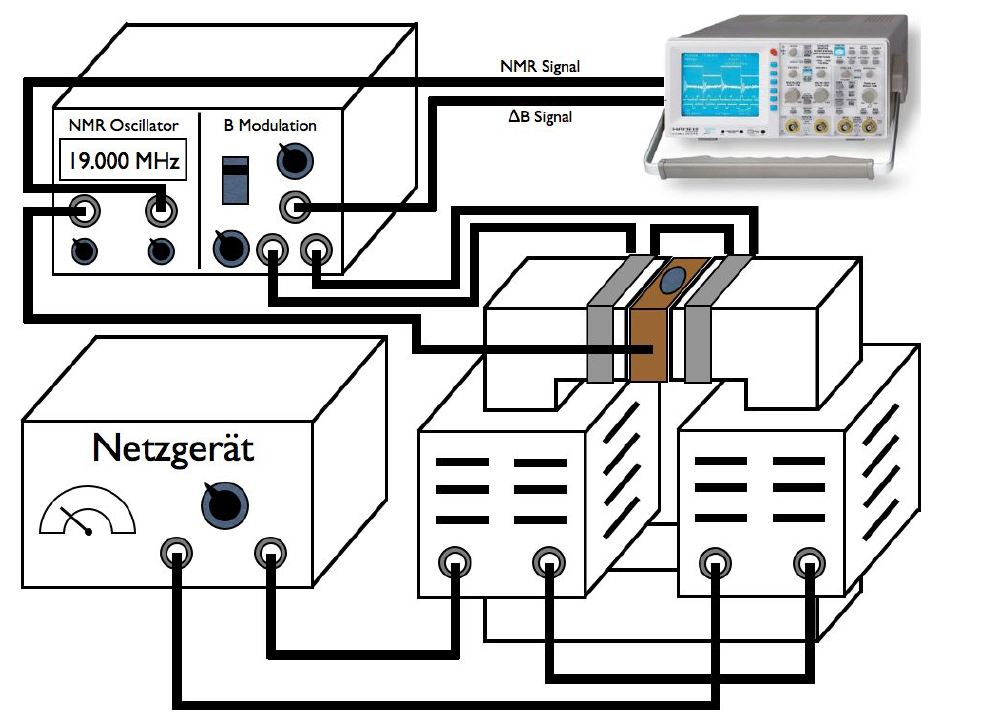
\includegraphics[scale=0.8]{Bild/Setup1}
	\centering
	\caption[Block Diagram for Setup 1]{Setup for measuring the resonance frequency with a sinus modulation.}
	\label{Exp_part1}
\end{figure}
\subsubsection{Lock-In Method}
For the second part the lock-in method is used since it is more precise duo to its lower background noise. Instead of the former absorption curve this method gives the differentiated curve. For the modulation of the magnetic field the superposition of a sinus and a sawtooth is used. Here the sawtooth is used mainly for the variance of the field while the sinus is used to create the differentiated signal since it has a similar frequency to the reference signal. The former minima of the absorption curve will now be the 'Nulldurchgang' of the signal. The moment the 'Nulldurchgang' of both measured signals overlap the correct resonance frequency is hit. Examples of both signals are shown in figure \ref{SägezahnBsp} and the setup is given in figure \ref{Exp_part2}.
\begin{figure}[ht]
	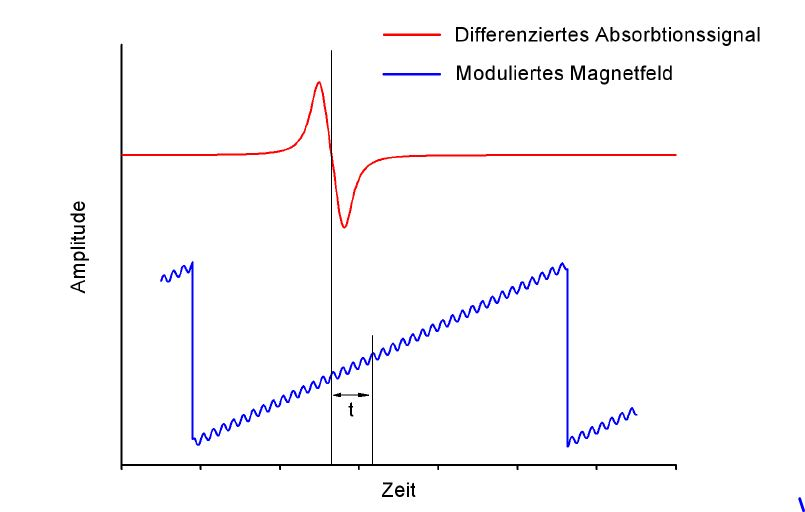
\includegraphics[scale=0.8]{Bild/BspLockIn}
	\centering
	\caption{Derived absorption signal in red. Superposition of sinus and sawtooth waves with both 'Nulldurchgängen' aligned.}
	\label{SägezahnBsp}
\end{figure}
\begin{figure}[ht]
	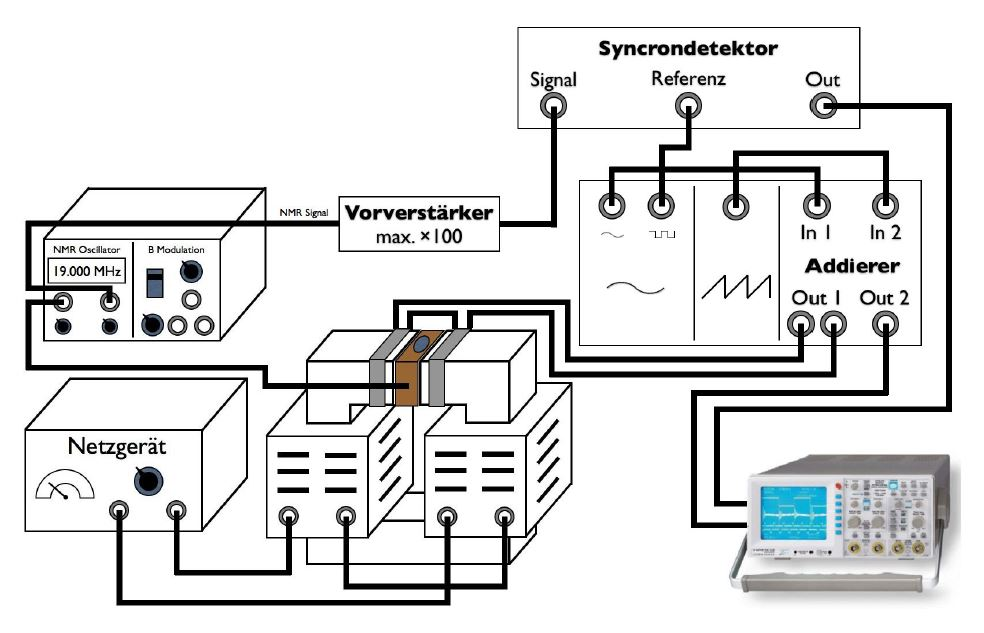
\includegraphics[scale=0.8]{Bild/Setup2}
	\centering
	\caption[Block Diagram for Setup 2]{Setup for measuring the resonance frequency with the lock-in method.}
	\label{Exp_part2}
\end{figure}


	\section{Durchführung des Versuches}
Vor der mündlichen Abfrage wurde die Messung vom Cobalt Spektrum mit dem CdTe Kristall gestartet mit einer Messzeit von einer Stunde. Nach der der mündlichen Abfrage wurde der CdTe Kristall gegen eine Silizium Diode getauscht und das zweite Cobalt Spektrum wurde mit der Messzeit von einer Stunde aufgenommen. \par
Während die obige Messung lief wurde mit den Vorbereitungen Absorptions- und Transmissionsmessungen zu Silizium gestartet. Es wurde der Strahlengang eingestellt und vorläufige Parameter des Lock-in Verstärkers gefunden.\par
Nun wurde auch das Cobalt Spektrum mittels der Silizium Diode aufgenommen, weshalb die Probe auf Americium gewechselt wurde und dessen Spektrum aufgezeichnet wurde. Die Messzeit betrug wieder eine Stunde.\par
Nach der ersten Testmessung zu Transmission und Absorption wurden die finalen Verstärkereinstellungen vorgenommen. Es wurden zwei normale Messungen und drei Untergrundmessungen aufgezeichnet: Eine ohne die Silizium Probe, eine ohne das Gitter und eine mit abgedunkeltem Spalt. Hierzu wurde das Gitter von $-90^{\circ}$ bis $+90^{\circ}$ gedreht und immer die Position des Gitters und der Widerstand der Probe sowie die Spannung des Pyrodetektors aufgezeichnet.\par
Nach Abschluss der ersten Americium Messung wurde klar, dass die Probe in der falschen Orientierung auf den Detektor platziert wurde, die Zählrate war viel niedriger als erwartet. Nachdem die Probe richtig platziert wurde, konnte die Messung mit Dauer einer Stunde erneut gestartet werden.\par
Da die Absorptions- und Transmissionsmessungen nun für Silizium abgeschlossen sind, wurde der Aufbau für die Germanium Probe vorbereitet: Das Gitter, der Filter und die Probe wurden vertauscht. Nun wurde der Verstärker für die Germanium Probe angepasst. Leider gab es zunächst Probleme, sodass man die realen Maxima erst bei maximaler Verstärkung finden konnte. Alls die Fehlersuche sich hinzog wurde beschlossen sich aufzuteilen und die Haynes und Shockley Messungen parallel durchzuführen.\par
Zunächst wurde der Offset von Glasfaser zu Elektrode bestimmt, anschließend wurde der Versuchsaufbau in Betrieb genommen. Es wurde nun die minimale Spannung  gefunden, bei welcher vermutet wurde, dass eine Auswertung der Messung in Form einer angepassten Gaußkurve möglich ist. Dann wurde in $2\,$V, später $4\,$V Schritten die Spannung erhöht bis zur maximal möglichen Spannung von $48\,$V.\par
Nun war die Messung des Americium Spektrums mit der Silizium Diode abgeschlossen und sie wurde gegen den CdTe Kristall getauscht. Anschließend wurde die letzte Messung gestartet. \par
Für das Haynes und Shockley Experiment wurden nun die Abstandsmessungen durchgeführt. Hierbei wurde zunächst die maximale Spannung an der Probe angelegt, und der Abstand so lange erhöht bis zur maximalen Distanz, bei welcher es für möglich gehalten wurde, eine Auswertung durchzuführen. Diese lag bei $9\,$mm auf der angebrachten Skala. Der Abstand wurde immer um einen mm zwischen den gespeicherten Messungen reduziert, bis zum minimalen Abstand von $2\,$mm. Es wurde nun noch einmal der Offset zwischen Glasfaser und Elektrode bestimmt, welcher jetzt $3.6\,$mm betrug. \par
Währenddessen wurde der Strahlenverlauf der Absorptions- und Transmissionsmessungen angepasst, sodass hier auch die oben erwähnten Messungen aufgenommen werden konnten.
	\section{Analyse der Energiespektren}
Da leider nicht alle Messungen über die selbe Zeit aufgenommen wurden, mussten diese über die Messdauer normiert werden, es wurden also immer die Zählraten anstatt der Counts verwendet. Diese Normierung wurde immer nach 
Berechnung der  statistischen Fehler des Datensatzes über die Formel \ref{zählfehler} durchgeführt. Die Fehler wurden nach der Formel \ref{fehlerfortp} fortgepflanzt.
\begin{equation}
\Delta_N = \sqrt{N}
\label{zählfehler}
\end{equation}
\begin{equation}
	\Delta_\frac{N}{t} = \frac{\Delta_N}{t} 
	\label{fehlerfortp}
\end{equation}
\subsection{Untergrund}
Zu Beginn wurde die Untergrundmessung ausgewertet, da diese benötigt wird um alle weiteren Messungen zu korrigieren. Es wurde statt einer langen Messung zwei kürzere aufgenommen, was durch addieren der Counts pro Bin behoben wurde.
Für die resultierende Datenreihe wurden wie oben beschrieben die statistischen Fehler berechnet und die Normierung durchgeführt. Die zur Hintergrundkompensation genutzte Datenreihe ist in Abbildung \ref{untergrund} zu sehen.
\begin{figure}[h]
	\centering
	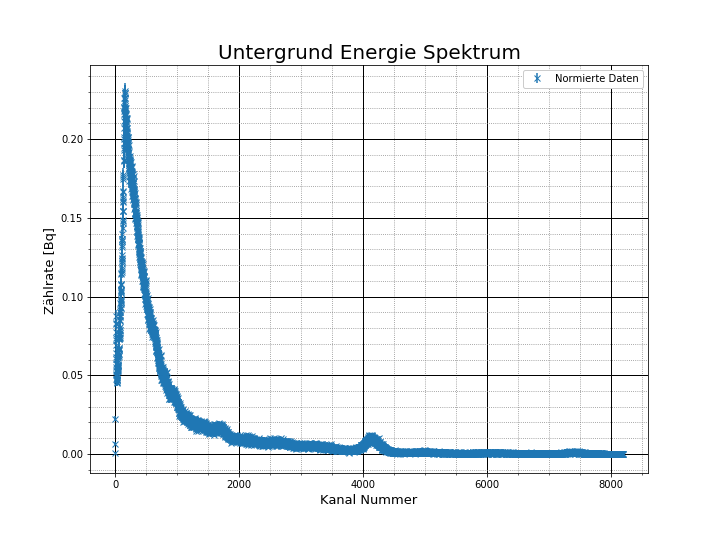
\includegraphics[scale=0.5]{Bilder/untergrund}
	\caption[Normalisierter Hintergrund]{\small Im Bild ist der Hintergrund Datensatz zu sehen. Es wurde die Zählrate pro Kanal aufgetragen. }
	\label{untergrund}
\end{figure}
\subsection{Energiekalibrierung}
Um den aktuellen Zusammenhang zwischen Kanälen des MCA und Energie der Detektierten $\gamma$ Photonen zu bestimmen, wurden die bekannten Peaks der Spektren von Natrium, Cobalt und Europium verwendet. Die so gewonnenen Zusammenhänge wurden auf den gesamten Bereich extrapoliert. Es wurden immer die statistischen Fehler in den Fits berücksichtigt.
\subsubsection{Natrium}
Für das Spektrum der $^{22}Na$ Probe wurden zwei Peaks erwartet, die Intensität des mit niedrigerer Energie einen deutlich größer als die des höher energetischen Peaks. Genau dies wurde beobachtet, somit konnten erfolgreich die Kanal-Energie Zusammenhänge für den 511 und 1275 keV Peak bestimmt werden. Hierzu wurden zunächst Analog zur Hintergrundmessung die statistischen Fehler bestimmt und die Counts in die Zählrate umgerechnet. 
Anschließend wurde eine Gaußkurve (nach Gleichung \ref{gaussian}) mittels Python \cite{SciPy_Opti} gefittet. Die Mittelpunkte der Peaks ($\mu$), welche für die Kalibrierung verwendet wurden sind der Abbildung \ref{natrium} zu entnehmen. 
\begin{figure}[h]
	\centering
	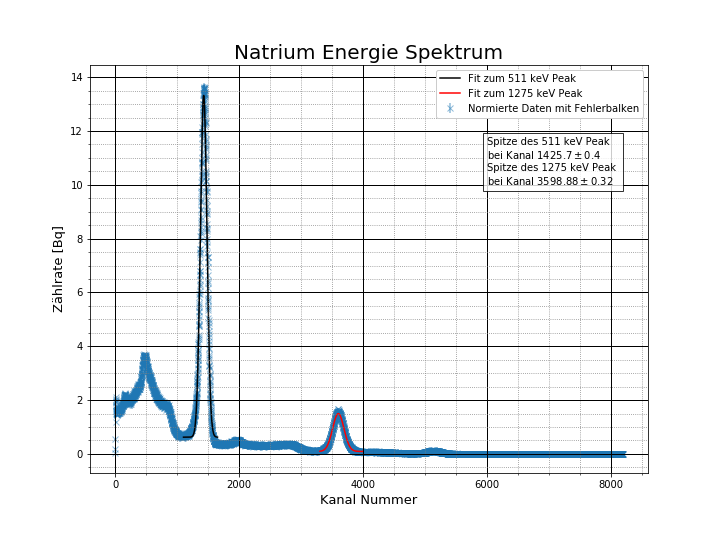
\includegraphics[scale=0.5]{Bilder/Natrium}
	\caption[Natriumspektrum mit Peaks]{\small Im Bild ist das Natrium Spektrum zu sehen. Es wurde die Zählrate pro Kanal aufgetragen und die Fits eingezeichnet. Zusätzlich sind die $\mu$ Werte der gefitteten Kurven eingetragen.}
	\label{natrium}
\end{figure}
\begin{equation}
f(x,\mu, \sigma, A, B) = B + A \cdot e ^{-\frac{(x - \mu) ^ 2}{2 \cdot \sigma ^ 2}}
\label{gaussian}
\end{equation}
\subsubsection{Cobalt}
Für das zur Kalibrierung verwendete Spektrum von $^{60}Co$ wurde analog zur Analyse des Natriumspektrums vorgegangen. Hier wurden zwei Peaks mit den Energien 1173 und 1333 keV erwartet. Diese konnten ohne größere Probleme gefunden und gefittet werden. Die relevanten Werte sind aus Abbildung \ref{cobalt} zu entnehmen. 
\begin{figure}[h]
	\centering
	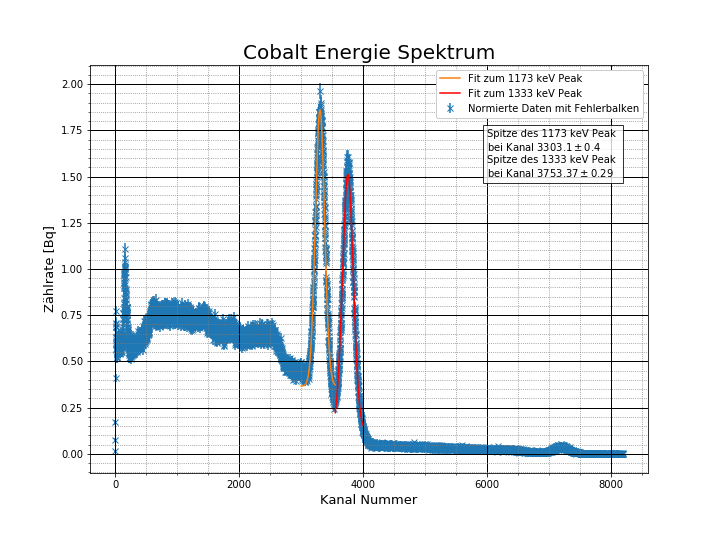
\includegraphics[scale=0.5]{Bilder/Cobalt}
	\caption[Cobalt Spektrum mit Peaks]{\small Im Bild ist das Cobalt Spektrum zu sehen. Es wurde die Zählrate pro Kanal aufgetragen und die Fits eingezeichnet. Zusätzlich sind die $\mu$ Werte der gefitteten Kurven eingetragen.}
	\label{cobalt}
\end{figure}
\subsubsection{Europium}
Durch die höhere Komplexität des Zerfalls von $^{152}Eu$ wurden im gemessenen Spektrum viele Peaks aufgezeichnet. Mit der Natriummessung als Referenz konnten die ungefähren Kanäle für die Energien von 122 und 344 keV bestimmt werden und analog zu den anderen beiden Messungen die Auswertung durchgeführt werden. Die relevanten Werte sind aus Abbildung \ref{europium} zu entnehmen. Durch

\begin{figure}[h]
	\centering
	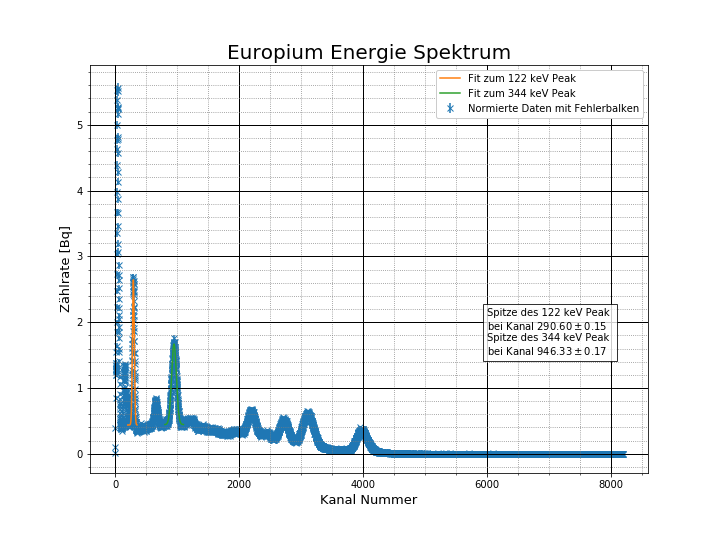
\includegraphics[scale=0.5]{Bilder/Europium}
	\caption[Europium Spektrum mit Peaks]{\small Im Bild ist das Europium Spektrum zu sehen. Es wurde die Zählrate pro Kanal aufgetragen und die Fits eingezeichnet. Zusätzlich sind die $\mu$ Werte der gefitteten Kurven eingetragen.}
	\label{europium}
\end{figure}
\subsubsection{Energieeichung}
Die in den vorherigen Abschnitten gewonnenen Energie-Kanal paare wurden nun aufgetragen und eine Linie wurde gefittet. Diesen Fit und die Parameter können in Abbildung \ref{energiekali} gefunden werden. Beim fit wurden die Fehler der Kanalnummer berücksichtigt, da die Energien ohne Fehler angenommen werden.

\begin{figure}[h]
	\centering
	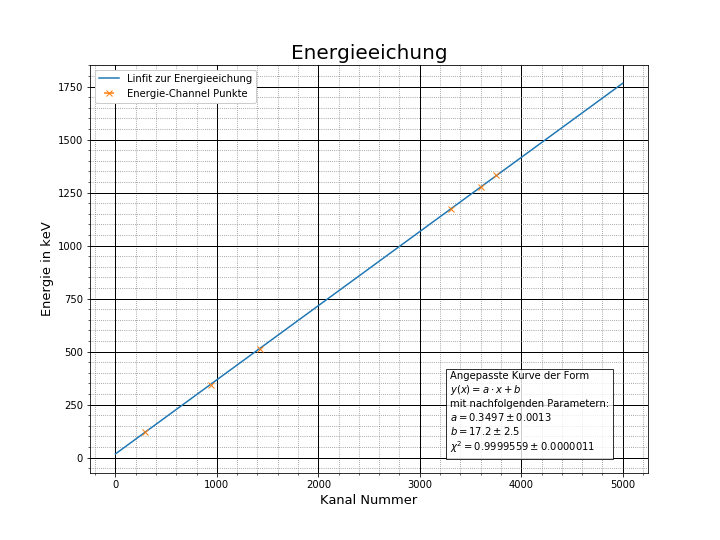
\includegraphics[scale=0.5]{Bilder/Energieeichung}
	\caption[Energieeichung]{\small Hier wurden die Kanal-Energie Paare aufgetragen und eine Kurve gefittet. Die Funktion und deren Parameter sowie die Güte sind zusätzlich eingetragen. }
	\label{energiekali}
\end{figure}

\subsection{Thorium Spektrum}
Das $^{228}Th$ Spektrum ist viel komplexer als die vorherigen. Es wurden 9 Peaks gefittet, wobei die Abbildungen hierzu im Anhang zu finden sind. Der 3. Peak ist ein Doppelpeak, sodass nicht die übliche Funktion (\ref{gaussian}) sondern eine Kombination aus zwei solcher Funktionen (\ref{doppelgaus}) gefittet wurde. Es wurde auch weiterhin Python \cite{SciPy_Opti} verwendet. Es wurden weiterhin die Statistischen Fehler berücksichtigt, da die Fehler auf die Energie viel kleiner sind.
\begin{equation}
	f(x,\mu,\mu_2,\sigma,\sigma_2,A,A_2,B) = 
	 A \cdot e ^{-\frac{(x - \mu) ^ 2}{2 \cdot \sigma ^ 2}} + 
	 A_2 \cdot e ^{-\frac{(x - \mu_2) ^ 2}{2 \cdot \sigma_2 ^ 2}} + 
	 B
	 \label{doppelgaus}
\end{equation}
In Abbildung \ref{thorium} ist das gesamte Thorium Spektrum in Logarithmischer Skala aufgetragen. Anschließend wurden kleinere Ausschnitte aufgetragen, dass die einzelnen Peaks besser erkennbar sind. Im Spektrum bis 500 keV (Abb. \ref{th_500}) wurden alle 5 Peaks gefittet. Im Spektrum von 500 bis 1000 keV (Abb. \ref{th_1000}) wurden alle 3 gut sichtbaren Peaks gefittet. Am Ende wurde noch der gut sichtbare Peak bei $\approx 3700$ keV gefittet. Die Energien der gefitteten Peaks sind auf den Abbildungen der jeweiligen Peaks in der Zuordnung zu finden
Die Mittelpunkte ($\mu$) der gefitteten Kurven wurden in der Tabelle \ref{ergebnisse_thorium} eingetragen. 
\begin{figure}[h]
	\centering
	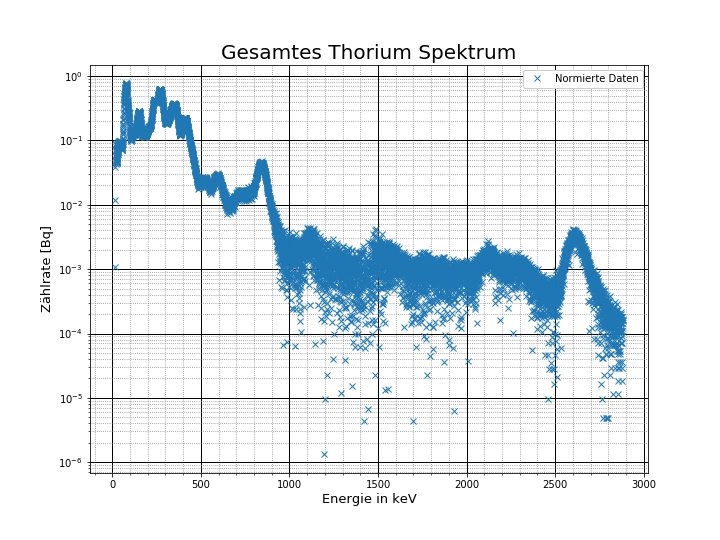
\includegraphics[scale=0.7]{Bilder/Th_ganz}
	\caption[Gesamtes Thorium Spektrum]{\small Thorium Spektrum in log. Skala, sodass alle Peaks mit stark variierenden Zählraten sichtbar sind.}
	\label{thorium}
\end{figure}

\begin{figure}[h]
	\centering
	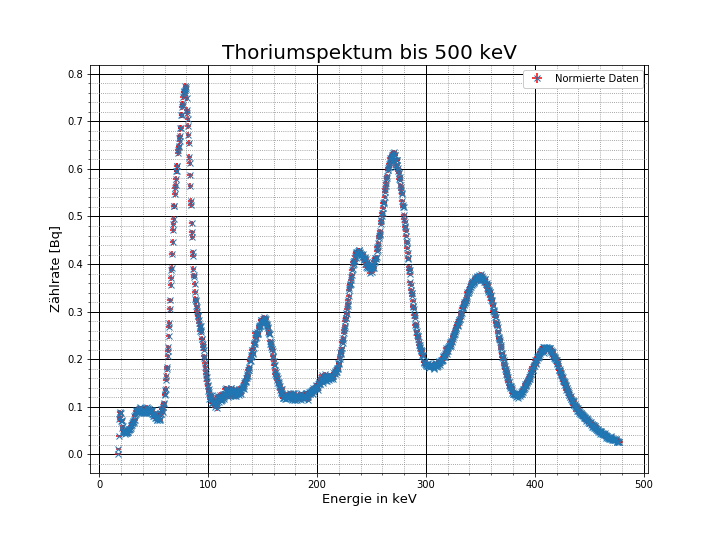
\includegraphics[scale=0.7]{Bilder/Th_1}
	\caption[Thorium Spektrum bis 500 keV]{\small Thorium Spektrum in lin. Skala bis 500 keV. Es sind die Peaks 1 bis 5 sichtbar, wobei Peak 3 ein Doppelpeak ist. Es wurde die Fehlerbalken zur Übersicht nicht bei allen Punkten eingezeichnet, die Energiefehler sind außerdem zu klein um dargestellt zu werden.}
	\label{th_500}
\end{figure}

\begin{figure}[h]
	\centering
	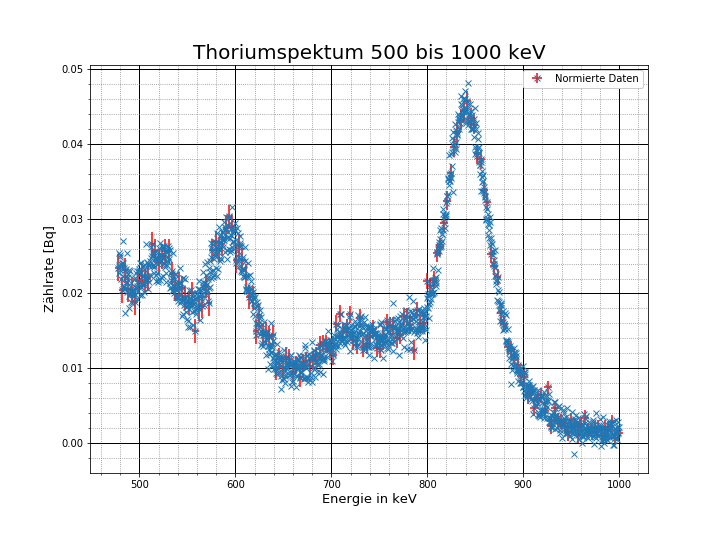
\includegraphics[scale=0.7]{Bilder/Th_2}
	\caption[Thorium Spektrum 500 bis 1000 keV]{\small Thorium Spektrum in lin. Skala von 500 bis 1000 keV. Es sind die Peaks 6 bis 8 sichtbar.
	Es wurde die Fehlerbalken zur Übersicht nicht bei allen Punkten eingezeichnet, die Energiefehler sind außerdem zu klein um dargestellt zu werden.}
	\label{th_1000}
\end{figure}
 \FloatBarrier
\subsection{Identifizierung der gemessenen Peaks}
Im Anschluss an die Bestimmung der Energien von den 10 verschiedenen Peaks (vgl. oben) wurden diese mit der Zerfallsreihe von Thorium verglichen um so die Übergänge zu Identifizieren bei welchen die gezählten $\gamma$ Photonen erzeugt wurden.
\subsubsection{Peak 1}
Peak 1 wurde bei einer Energie von $77.26\pm0.10\,$keV gefittet. 
Beim Blick auf Abbildung \ref{p1} ist auffällig, dass der Peak unsauber ist, als ob er bei ca. 72 keV einen weiteren Peak besitzt, was den gesamten Fit verzieht. Das echte Maximum von Peak 1 liegt außerdem bei einer deutlich höheren Energie als das Maximum des Fits. Deshalb wird es als sinnvoll empfunden, einen anderen Mittelpunkt und ein größerer Fehler auf diesen Wert angenommen: Der neue Wert liegt nun bei $80\pm5\,$keV.\par
Wahrscheinlich handelt es sich hier um den Übergang von Thorium zu Radium mit Energie 84.373 keV \cite{Thorium}. Von der Energie würde zusätzlich noch der Übergang Thorium zu Radium bei 74.4 keV, möglich sein, was vermutlich den Peak leicht zu einer niedrigeren Energie verschob.
\begin{figure}[h]
	\centering
	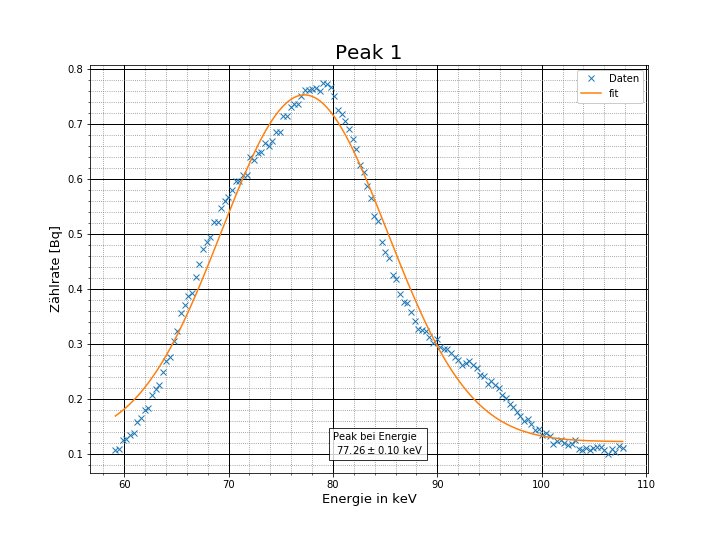
\includegraphics[scale=0.7]{Bilder/Anhang/P1}
	\caption[Thorium Peak 1]{\small Die verwendeten Daten von Peak 1, dessen Fit und der Mittelpunkt des Fits.}
	\label{p1}
\end{figure}
\FloatBarrier
\subsubsection{Peak 2}
Das Maximum von Peak 2 wurde bei einer Energie von $149.67\pm0.08\,$keV gefittet. Dies ist aus Abbildung \ref{p2}. Durch die hohe Streuung in der Umgebung des Maximums wird es für sinnvoll gehalten, den Fehler zu vergrößern: Somit gilt nun für den Mittelpunkt des Fits die Energie von $150\pm5\,$keV.\par
Bei dieser Energie liegt kein direkter Peak vor, aber es existieren die Übergänge 131.612 keV  und 166.41 keV  von Thorium zu Radium \cite{Thorium} . Deshalb wird vermutet, dass der gemessene Peak eine Kombination von beiden sei, welche wegen den Unterschiedlichen Wahrscheinlichkeiten der Übergänge nicht mittig zwischen ihnen liegt, sondern etwas näher an 166.41 keV.
\begin{figure}[h]
	\centering
	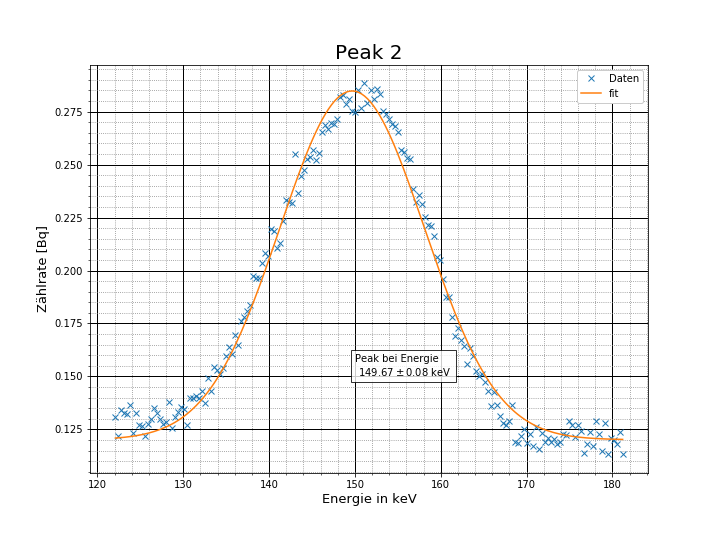
\includegraphics[scale=0.7]{Bilder/Anhang/P2}
	\caption[Thorium Peak 2]{\small Die verwendeten Daten von Peak 2, dessen Fit und der Mittelpunkt des Fits.}
	\label{p2}
\end{figure}
\FloatBarrier
\subsubsection{Peak 3}
Peak 3 war ein Kombinationspeak. Deshalb werden die beiden Komponenten von ihm einzeln als 3.1 und 3.2 betrachtet. Dies ist alles in Abbildung \ref{p3} zu sehen.\\
Das gefittete Maximum von Peak 3.1 liegt bei $237.62\pm0.10\,$keV. Da der Kombinationsfit in dieser Region deutlich über der Mehrheit der Punkte liegt, wurde es für sinnvoll erachtet den Fehler auf einen größeren Wert festzulegen: Für Peak 3.1 gilt nun $238\pm2\,$keV.\\
Das gefittete Maximum von Peak 3.2 liegt bei $269.88\pm0.06\,$keV. Da hier am Peak eine gewisse Streuung der Messpunkte vorliegt, wird auch ein vergrößerter Fehler angenommen: Somit gilt für Peak 3.2 nun eine Energie von
$270\pm1\,$keV. Vermutlich spielen hier außerdem Überlagerungen von Comptoneffekten der darüberlegenden Peaks eine Rolle, weshalb zusätzlich systematische Fehler anzunehmen sind. \cite{staatsex_szinti} \par
Für die Energie zu Peak 3.1 passt der Übergang von Blei zu Bismut \cite{Blei} mit einer Energie von 238.632 keV. Für Peak 3.2 passt der Übergang von Thallium zu Blei bei 277.37 keV \cite{Thallium} am Wahrscheinlichsten. 


\begin{figure}[h]
	\centering
	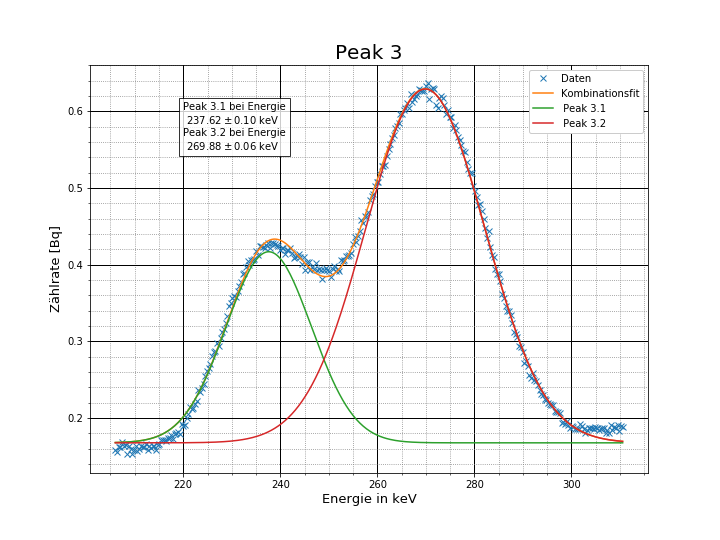
\includegraphics[scale=0.7]{Bilder/Anhang/P3}
	\caption[Thorium Peak 3]{\small Die verwendeten Daten von Peak 3, der gefittete Kombinationspeak, die einzelnen Peaks und ihre Mittelpunkte.}
	\label{p3}
\end{figure}
\FloatBarrier
\subsubsection{Peak 4}
Das gefittete Maximum von Peak 4 liegt bei $345\pm0.23\,$ keV, was Abbildung \ref{p4} zu entnehmen ist. Es ist relativ offensichtlich, dass hier das echte Maximum der Daten neben dem des Fits liegt, weshalb für die Energie von Peak 4 der Wert $350\pm3\,$ keV angenommen wird. Vermutlich spielen hier außerdem Überlagerungen von Comptoneffekten der darüberlegenden Peaks eine Rolle, weshalb zusätzlich systematische Fehler anzunehmen sind \cite{staatsex_szinti}.\par
Hier existert kein Zerfall mit ähnlicher Energie zu Peak 4. Der nächste Übergang wäre der von Bismut zu Thallium bei einer Energie von 327.94 keV \cite{Bismut}. 
\begin{figure}[h]
	\centering
	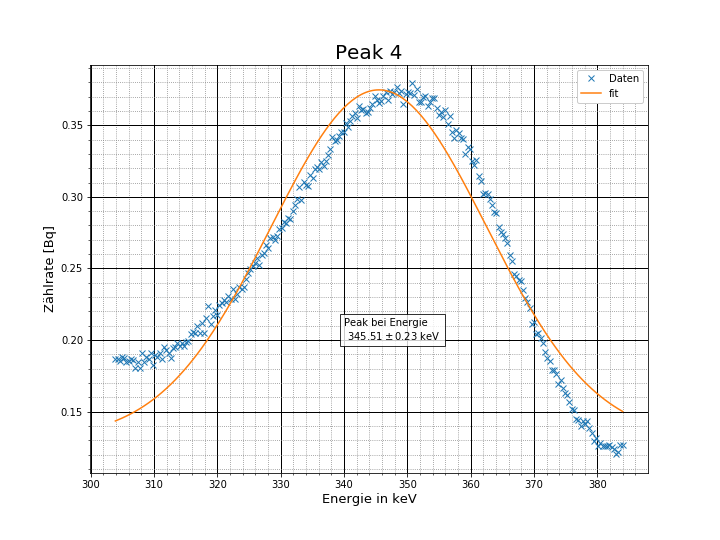
\includegraphics[scale=0.7]{Bilder/Anhang/P4}
	\caption[Thorium Peak 4]{\small Die verwendeten Daten von Peak 4, der gefittete Peak und sein Mittelpunkt.}
	\label{p4}
\end{figure}
\FloatBarrier
\subsubsection{Peak 5}
Das gefittete Maximum von Peak 5 liegt bei $409.99\pm0.07\,$keV nach Abbildung \ref{p5}. Durch die hohe Streuung der Messwerte sollte ein höherer Fehler auf diesen Wert Angenommen werden, sodass für den Peak der Wert $410\pm2\,$keV gilt.\par
Hier wurde wahrscheinlich der Übergang von Blei zu Bismut mit einer Energie von 415.27 keV \cite{Blei} gemessen. 

\begin{figure}[h]
	\centering
	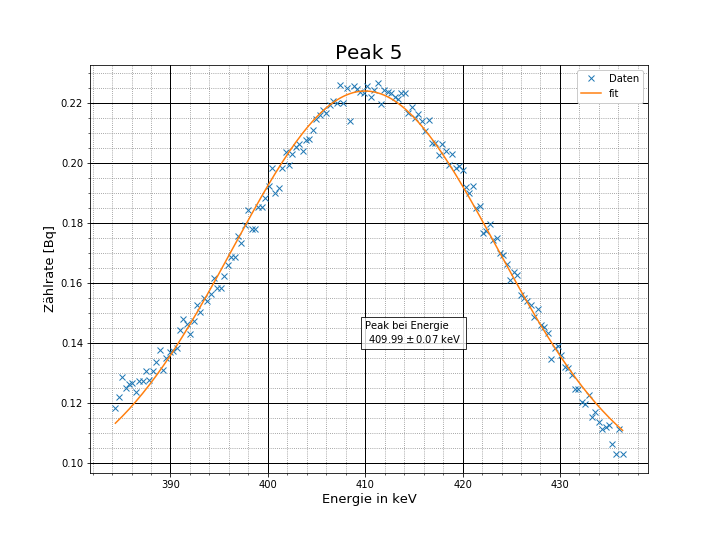
\includegraphics[scale=0.7]{Bilder/Anhang/P5}
	\caption[Thorium Peak 5]{\small Die verwendeten Daten von Peak 5, der gefittete Peak und sein Mittelpunkt.}
	\label{p5}
\end{figure}
\FloatBarrier
\subsubsection{Peak 6}
Das gefittete Maximum von Peak 6 liegt bei $518.8\pm0.9\,$keV nach Abbildung \ref{p6}. Durch die hohe Streuung der Messwerte ist ein größerer Fehler auf diesen Wert angenommen worden, sodass für den Peak der Wert $519\pm5\,$keV gilt.\par
Wahrscheinlich wurde hier der 510.7 keV \cite{Thallium} Übergang von Thallium zu Blei gemessen.

\begin{figure}[h]
	\centering
	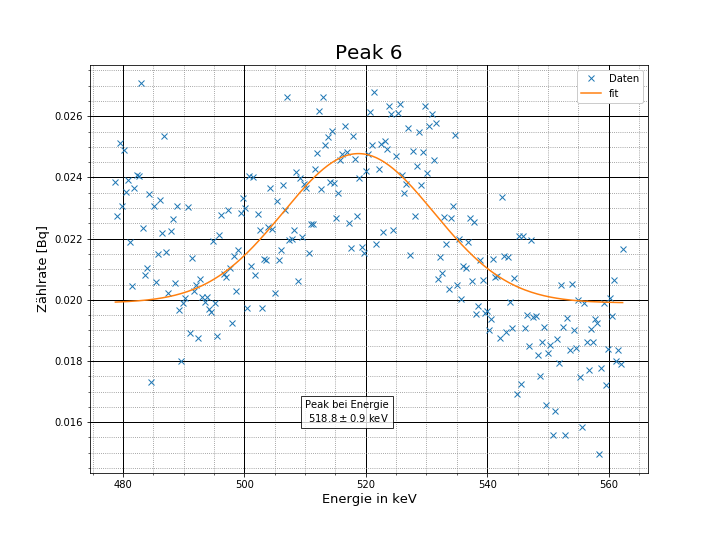
\includegraphics[scale=0.7]{Bilder/Anhang/P6}
	\caption[Thorium Peak 6]{\small Die verwendeten Daten von Peak 6, der gefittete Peak und sein Mittelpunkt.}
	\label{p6}
\end{figure}
\FloatBarrier
\subsubsection{Peak 7}
Das gefittete Maximum von Peak 7 liegt bei $591.04\pm0.31\,$keV nach Abbildung \ref{p7}. Durch die hohe Streuung der Messwerte ist ein größerer Fehler auf diesen Wert angenommen worden, sodass für den Peak der Wert von $591\pm5\,$keV gilt.\par
Wahrscheinlich wurde hier der 587.8 keV \cite{Thallium} Übergang von Thallium zu Blei gemessen.

\begin{figure}[h]
	\centering
	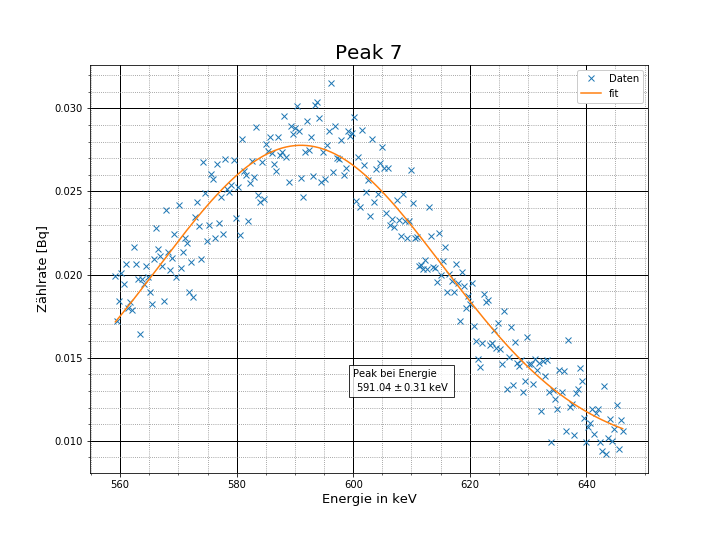
\includegraphics[scale=0.7]{Bilder/Anhang/P7}
	\caption[Thorium Peak 7]{\small Die verwendeten Daten von Peak 7, der gefittete Peak und sein Mittelpunkt.}
	\label{p7}
\end{figure}
\FloatBarrier
\subsubsection{Peak 8}
Das gefittete Maximum von Peak 8 liegt bei $839.44\pm0.15\,$keV nach Abbildung \ref{p8}. Durch die hohe Streuung der Messwerte wurde ein größerer Fehler auf diesen Wert angenommen, sodass für den Peak ein Wert von $839\pm5\,$keV gilt.\par
Wahrscheinlich wurde hier der 835.9 keV \cite{Thallium} von Thallium zu Blei gemessen.

\begin{figure}[h]
	\centering
	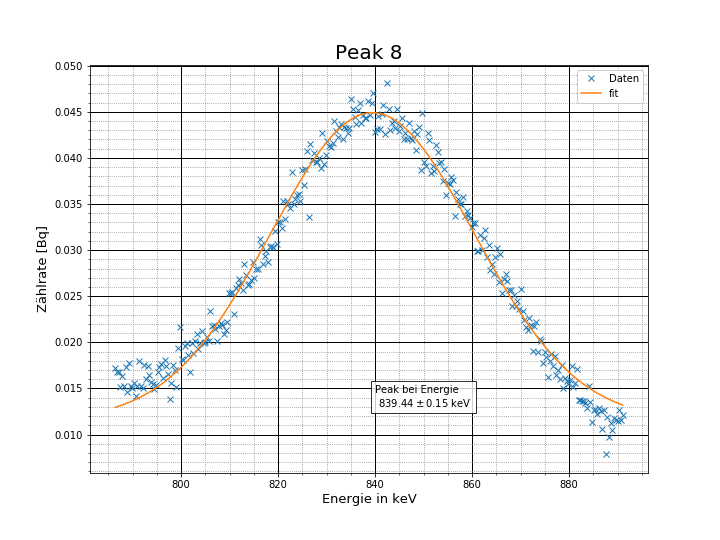
\includegraphics[scale=0.7]{Bilder/Anhang/P8}
	\caption[Thorium Peak 8]{\small Die verwendeten Daten von Peak 8, der gefittete Peak und sein Mittelpunkt.}
	\label{p8}
\end{figure}

\subsubsection{Peak 9}
Das gefittete Maximum von Peak 9 liegt bei $2614.1\pm0.5\,$keV nach Abbildung \ref{p9}. Durch die hohe Streuung der Messwerte wurde ein größerer Fehler auf diesen Wert angenommen, sodass für den Peak ein Wert von $2614\pm10\,$keV gilt.\par
Wahrscheinlich wurde hier der 2614.511 keV \cite{Thallium} Übergang von Thallium zu Blei gemessen.

\begin{figure}[h]
\centering
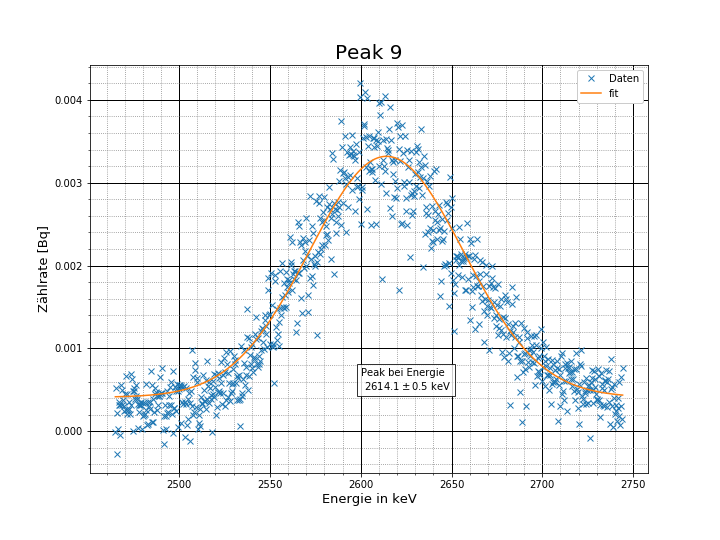
\includegraphics[scale=0.7]{Bilder/Anhang/P9}
\caption[Thorium Peak 9]{\small Die verwendeten Daten von Peak 9, der gefittete Peak und sein Mittelpunkt.}
\label{p9}
\end{figure}
\FloatBarrier
	\section{Auswertung der Winkelabhängigen Messung}
	\section{Diskussion der Ergebnisse}
\subsection{Energiespektren}
Während der Hintergrundmessung (Abb. \ref{untergrund}) viel nach dem ersten Peak, welcher durch die Messtechnik erklärbar ist, ein weiterer Peak mit der Spitze bei Kanal $4133.4\pm1.3$ erkennbar (Abb. \ref{untergrund_peak}).
\begin{figure}[h]
	\centering
	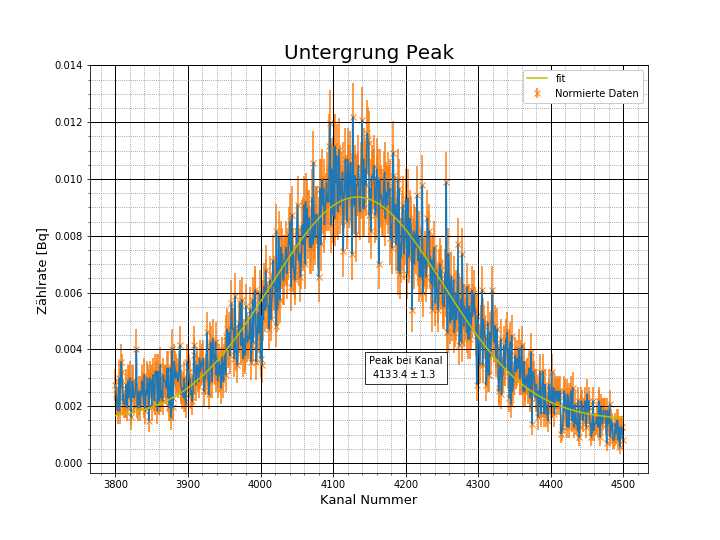
\includegraphics[scale=0.5]{Bilder/untergrund_peak}
	\caption[Peak im Hintergrund]{\small Im Bild ist der Peak im  Hintergrund Datensatz, dessen Fit und der Mittelpunkt des Fits zu sehen. Es wurde die Zählrate pro Kanal aufgetragen.}
	\label{untergrund_peak}
\end{figure}
Der Kanal im Peak wurde nach Gleichung \ref{energie-kanal} in den Kalibrierten Energiewert von $1463 \pm 6\,$keV, was in der Nähe des Übergangs von $^{40}K$ zu $^{40}Ca$ mit 1312.1 keV \cite{staatsex_szinti}. Nach der Formel \ref{vertrag} liegen diese jedoch bei einer Kompatibilität von 25 Standartabweichungen. Dies legt nahe, dass es sich um einen anderen Zefall handeln sollte. Dennoch ist dies die einzige Theorie, welche wir haben da alle im Versuch verwendeten Proben während der Messung stark abgeschirmt waren. Die Kalium Probe jedoch ist ein Pulver, welches im Versuch Lange Halbwertszeiten verwendet wird, welcher sich in räumlicher Nähe zum Versuchsaufbau befindet.\par
\begin{equation}
t = \frac{\left|x-y\right|}{\Delta_x}
\label{vertrag}
\end{equation}
Die Fits zu den Kalibriermessungen liefen Problemlos, die Resultierende Energieeichung des MCA lief auch gut, was am hohen $\chi^2$ Wert erkennbar ist.\par
Bei der Analyse des Thorium Spektrums fiel jedoch auf, dass obwohl der Fit zum jeweiligen Peak optisch nicht sehr gut passte, der Fehler auf den Parameter zum Maximum relativ klein war.
Bei der Zuordnung von den gefitteten Peaks zu den Übergängen der Thorium Zerfallsreihe viel auf, dass sehr viele Übergänge möglich waren, jedoch die meisten relativ unwahrscheinlich. Es ist dennoch nicht auszuschließen dass die gemessenen Übergänge durch zusätzlich die unwahrscheinlicheren Übergänge enthalten. Eine Analyse der 10 gefitteten Peaks des Thorium Spektrums mittels der Formel \ref{vertrag} ist in Tabelle \ref{Ergebnisse} zu erkennen.
\begin{table}
	\caption[Ergebnisse des Thorium Spektrums]{Die ermittelten Werte der Peaks des Thorium Spektrums sowie die Energien der zugeordneten Übergänge und deren Kompatibilität wurden in der nachfolgenden Tabelle aufgetragen.}
	\begin{tabular}{llll}
		\toprule
		{} & Gemessene Werte [keV] & Literaturwerte [keV] &                         Verträglichkeit \\
		\midrule
		Peak 1   &                80+/-5 &               84.373 &                                  0.8746 \\
		Peak 2   &               150+/-5 &    (131.612, 166.41) &  (3.7, 3.3) \\
		Peak 3.1 &           238.0+/-2.0 &              238.632 &                                   0.316 \\
		Peak 3.2 &           270.0+/-1.0 &               277.37 &                                    7.37 \\
		Peak 4   &           350.0+/-3.0 &               327.94 &                                 7.35333 \\
		Peak 5   &           410.0+/-2.0 &               415.27 &                                   2.635 \\
		Peak 6   &               519+/-5 &                510.7 &                                    1.66 \\
		Peak 7   &               591+/-5 &                587.8 &                                    0.64 \\
		Peak 8   &               839+/-5 &                835.9 &                                    0.62 \\
		Peak 9   &             2614+/-10 &              2614.51 &                                  0.0511 \\
		\bottomrule
	\end{tabular}
\label{Ergebnisse}
\end{table}
Es ist erkennbar, dass einige Werte relativ nahe an den Entsprechenden Literaturwerten liegen, andere jedoch weit von ihnen entfernt liegen. Dies ist insbesondere bei den Peaks 4 und 5 der Fall. Dies kann zum Teil durch Überlagerung von Comptoneffekten der darauffolgenden Peaks erklärt werden. Zusätzlich ist es sehr auffällig, dass die geschätzten Fehler groß sind, sodass die gemessenen Peaks teilweise sehr kleine Inkompatibilität haben. Dies ist vor allem bei Peak 9 der Fall, wo der gemessene Wert mit dem Literaturwert fast vollends übereinstimmt. 
\subsection{Winkelabhängige Messung}
Auch hier wurde die Kompatiblität des gemessenen Wertes von $-0.81\pm0.11\,$Grad mit dem erwarteten Wert von $0^\circ$ über die Formel \ref{vertrag} verglichen mit dem Ergebnis 7.4, wonach sie nicht kompatibel sind. Bei Betrachtung der Abbildung \ref{Winkelbild} fällt auf, dass im wichtigen Bereich die Datenpunkte vom Fit stark abweichen. Daraus kann man folgern, dass dieser Fit nicht repräsentativ für die Daten der Wichtigen Region ist. Bei Betrachtung der Daten einzeln fällt auf, dass mit Abstand die höchste Anzahl an Counts bei $0^\circ$ gemessen wurde, was darauf hinweist dass ein Problem mit dem Fit vorliegt.
	\section{Zusammenfassung}
Wenn man die gemessenen Werte mit denen des Literatur Wertes von $119\,$ns mit der Formel \ref{Vergleich} vergleicht erhält man die in Tabelle \ref{VglTable} beschriebenen Werte. \\
\begin{table}
	\begin{Dtabular}[1.1]{|c|c|c|}
		\hline
		Messreihe&Lebensdauer $\tau$[ns]&Vergleichswert\\
		\hline
		Abkühlen 1 bei $0^\circ$&$(1.224\pm0.022)$&\\
		\hline
		Abkühlen 1 bei $90^\circ$&&\\
		\hline
		Aufwärmen bei $0^\circ$&&\\
		\hline
		Abkühlen 2 bei $0^\circ$&&\\
		\hline
		Abkühlen 2 bei $90^\circ$&&\\
		\hline
	\end{Dtabular}
\end{table}
Man erkennt schnell, dass alle gemessenen Werte bis auf die Aufwärmmessung mit dem Literaturwert kompatibel sind. Die große Diskrepanz kann man dadurch erklären, dass für die Messung während des Aufwärmvorgangs nicht gewartet wurde bis die Temperatur des Thermometers mit der der Probe angeglichen hat. Dadurch ziehen wir einen großen systematischen Fehler mit welcher die Unverträglichkeit erklären könnte. \par Ein weiteres Problem ist sicher die geringe Anzahl an Messpunkten die wir in allen Messreihen hatten, wodurch sich natürlich unsere Messreihe verschlechtert. 

	\section{Bibliograpy}
	\bibliographystyle{plain}
	\bibliography{Quellen}
	\addcontentsline{toc}{section}{Literatur}
	\begin{figure}
	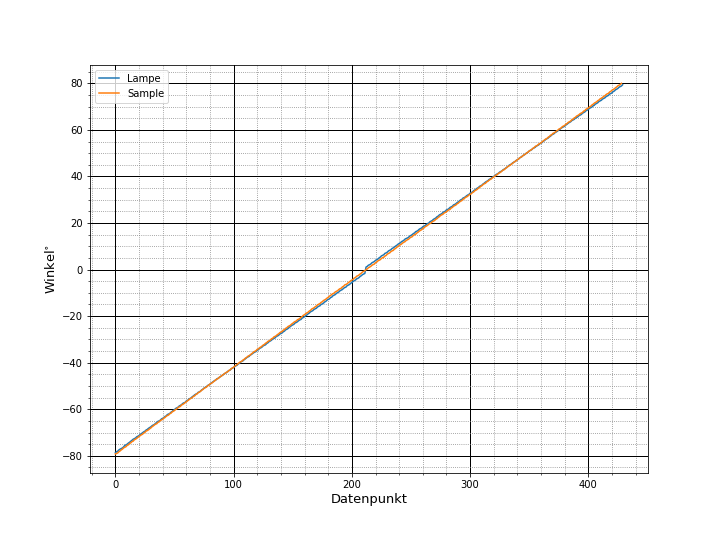
\includegraphics[scale=0.5]{Bilder/anhang/korrektur_channels_2}
	\centering
	\caption[Korrigierter Lampendatensatz 2. Silizium messung]{\small Auftragung der gemessenen Winkel für die Lampenmessung und erste Silizium Messung nach der Korrektur. Beide stimmen in den relevanten Bereichen bei ca. $30^{\circ}-40^{\circ}$ weitgehend überein.}
\end{figure}
\begin{figure}
	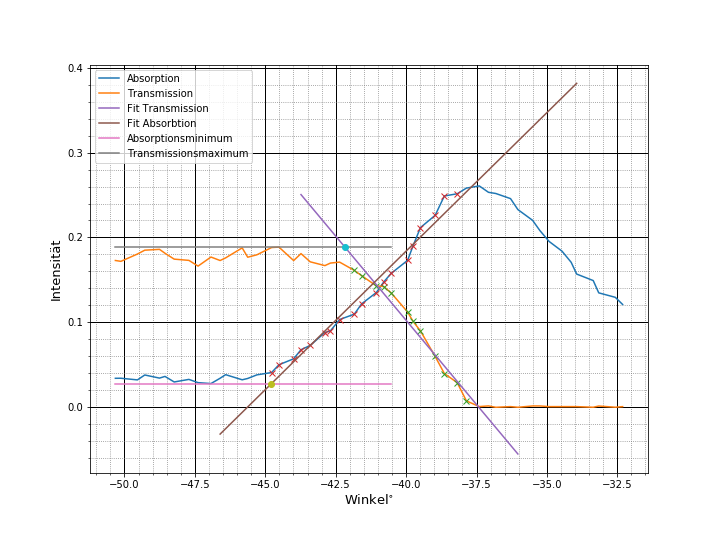
\includegraphics[scale=0.5]{Bilder/anhang/si_2_l}
	\centering
	\caption[Geraden Anpassungen 2. Silizium Messung links]{\small Auftragung von Intensität der normalisierten Datenreihen gegen die  Winkel in der Nähe der Stelle Gleichwahrscheinlicher Absorption und Transmission bei Winkeln kleiner als $0^\circ$. Es sind zusätzlich die angepassten Geraden zur Absorption und Transmission eingezeichnet. Die Horizontalen wurden durch die Maxima der dahinterliegenden Datenpunkte bestimmt. Die Schnittpunkte der Geraden mit ihren jeweiligen Horizontalen sind auch eingezeichnet.}
\end{figure}
\begin{figure}
	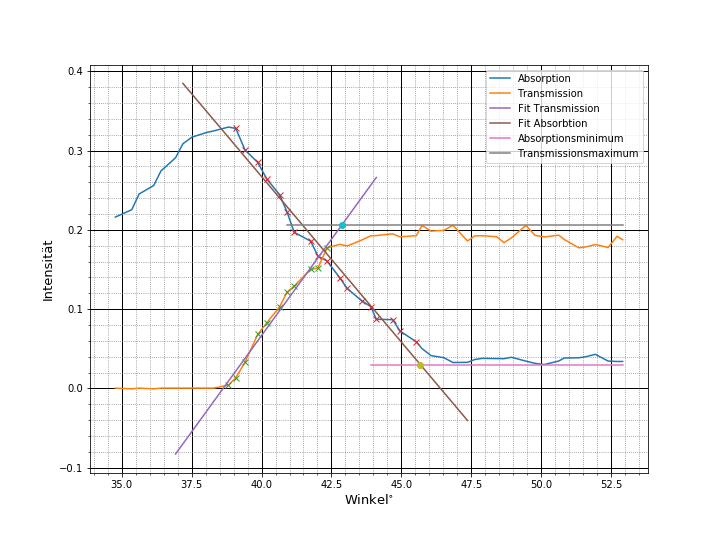
\includegraphics[scale=0.5]{Bilder/anhang/si_2_r}
	\centering
	\caption[Geraden Anpassungen 2. Silizium Messung rechts]{\small Auftragung von Intensität der normalisierten Datenreihen gegen die  Winkel der zweiten Silizium Messung in der Nähe der Stelle Gleichwahrscheinlicher Absorption und Transmission bei Winkeln größer als $0^\circ$. Es sind zusätzlich die angepassten Geraden zur Absorption und Transmission eingezeichnet. Die Horizontalen wurden durch die Maxima der dahinterliegenden Datenpunkte bestimmt. Die Schnittpunkte der Geraden mit ihren jeweiligen Horizontalen sind auch eingezeichnet.}
	\label{si_2_r}
\end{figure}
\begin{figure}
	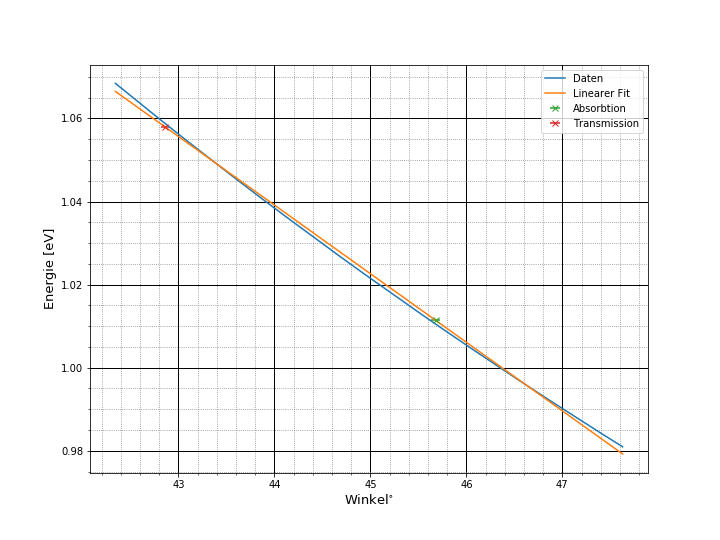
\includegraphics[scale=0.5]{Bilder/anhang/si_2_l_energie}
	\centering
	\caption[Energiebestimmung 2. Si Messung links]{\small Auftragung der Energie gegen den Winkel der zweiten Silizium Messung. Die angepasste Gerade und die beiden Schnittpunkte sind auch eingetragen.}
\end{figure}
\begin{figure}
	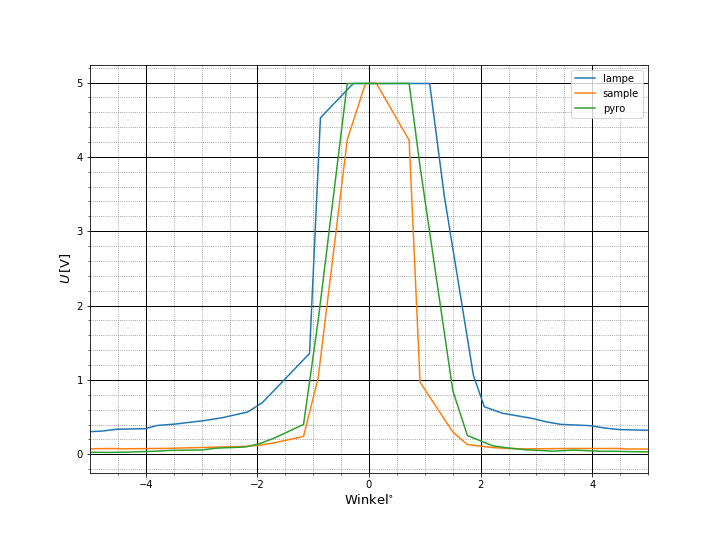
\includegraphics[scale=0.5]{Bilder/anhang/winkelkorrektur_vorher}
	\centering
	\caption[Mittelpunkt der 2. Si Messung vor Winkelkorrektur]{\small Auftragung der Intensität gegen den Winkel der zweiten Silizium Messung in der Nähe von $0^\circ$ vor der Korrektur.}
\end{figure}
\begin{figure}
	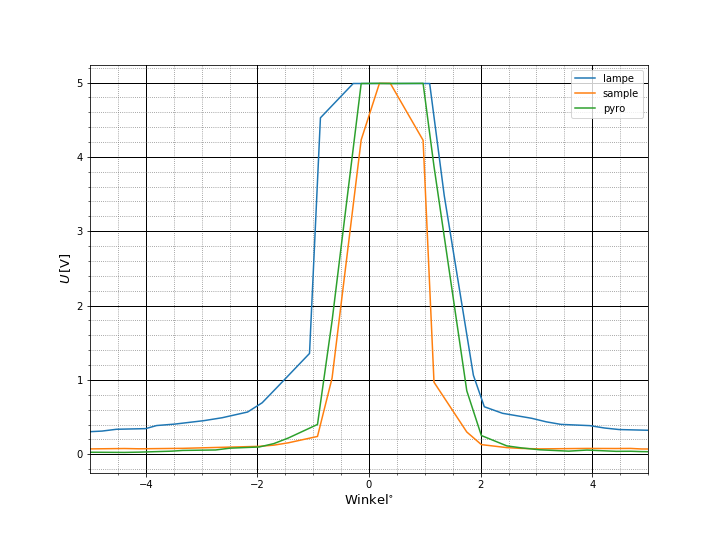
\includegraphics[scale=0.5]{Bilder/anhang/winkelkorrektur_nachher}
	\centering
	\caption[Mittelpunkt der 2. Si Messung vor Winkelkorrektur]{\small Auftragung der Intensität gegen den Winkel der zweiten Silizium Messung in der Nähe von $0^\circ$ nach der Korrektur.}
\end{figure}
\begin{figure}
	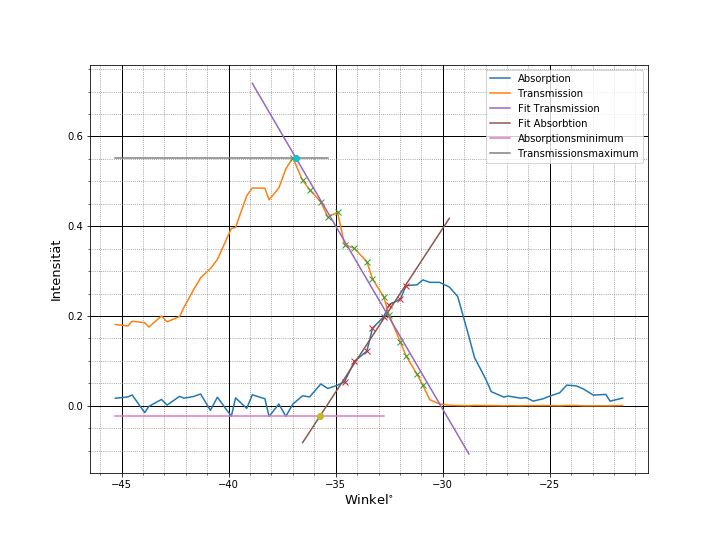
\includegraphics[scale=0.5]{Bilder/anhang/ge_r}
	\caption[Geraden Anpassungen Germanium Messung links]{\small Auftragung von Intensität der normalisierten Datenreihen von Germanium gegen die  Winkel in der Nähe der Stelle Gleichwahrscheinlicher Absorption und Transmission bei Winkeln größer als $0^\circ$. Es sind zusätzlich die angepassten Geraden zur Absorption und Transmission eingezeichnet. Die Horizontalen wurden durch die Maxima der dahinterliegenden Datenpunkte bestimmt. Die Schnittpunkte der Geraden mit ihren jeweiligen Horizontalen sind auch eingezeichnet.}
\end{figure}
\begin{figure}
	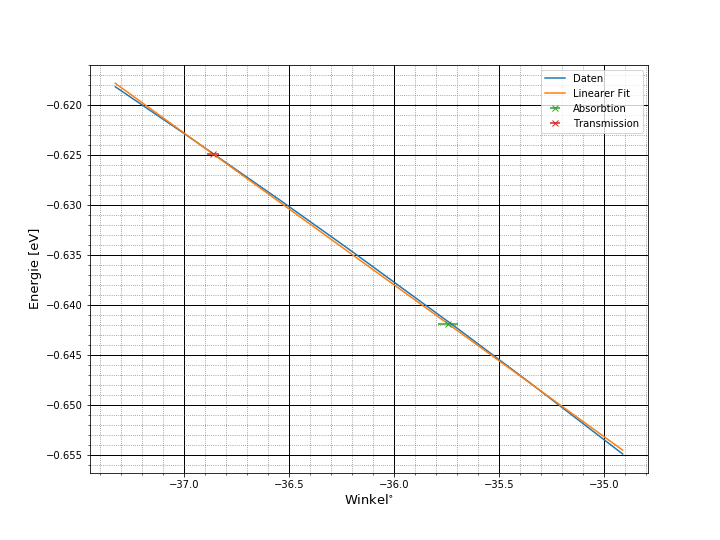
\includegraphics[scale=0.5]{Bilder/anhang/ge_l_energie}
	\centering
	\caption[Energiebestimmung Ge Messung links]{\small Auftragung der Energie gegen den Winkel der Germanium Messung. Die angepasste Gerade und die beiden Schnittpunkte sind auch eingetragen.}
\end{figure}


\begin{figure}
	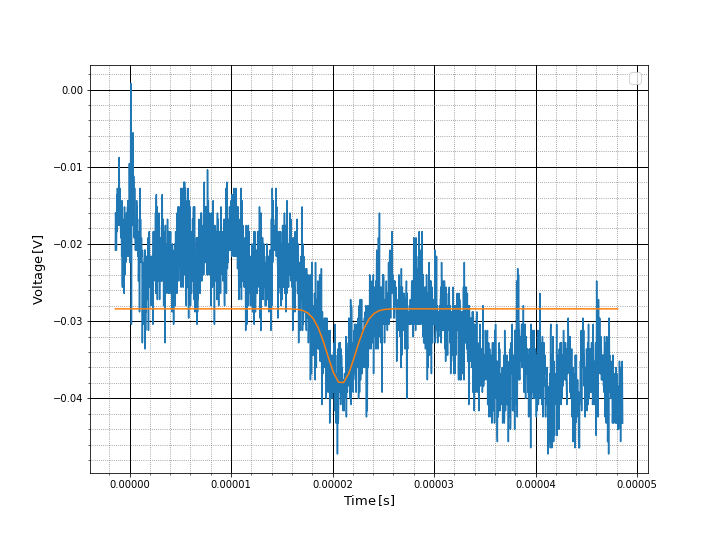
\includegraphics[scale=0.5]{Bild/S1}
	\centering
	\caption[Gaußfit an Messung bei Konst. Spannung 1]{Gaußfit an die Messungen der Elektronenwolken bei einer Spannung von $48\,$V und einem Abstand zwischen Nadel und Lase von $10.6$\,mm.}
\end{figure}
\begin{figure}
	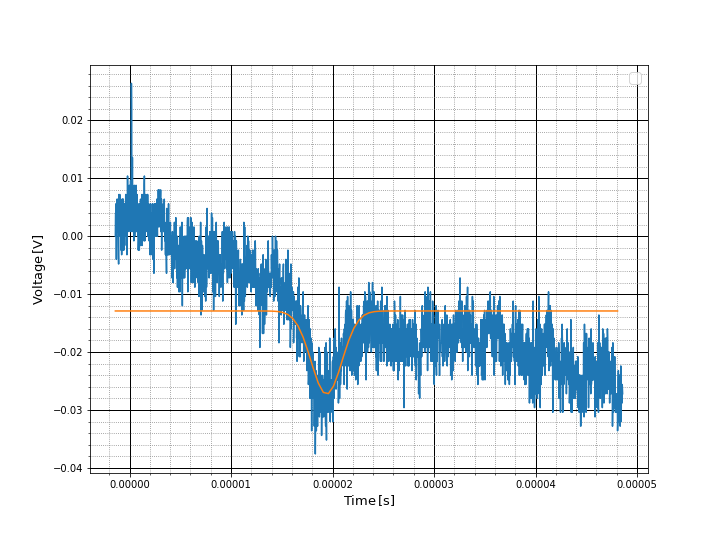
\includegraphics[scale=0.5]{Bild/S2}
	\centering
	\caption[Gaußfit an Messung bei Konst. Spannung 2]{Gaußfit an die Messungen der Elektronenwolken bei einer Spannung von $48\,$V und einem Abstand zwischen Nadel und Lase von $9.6$\,mm.}
\end{figure}
\begin{figure}
	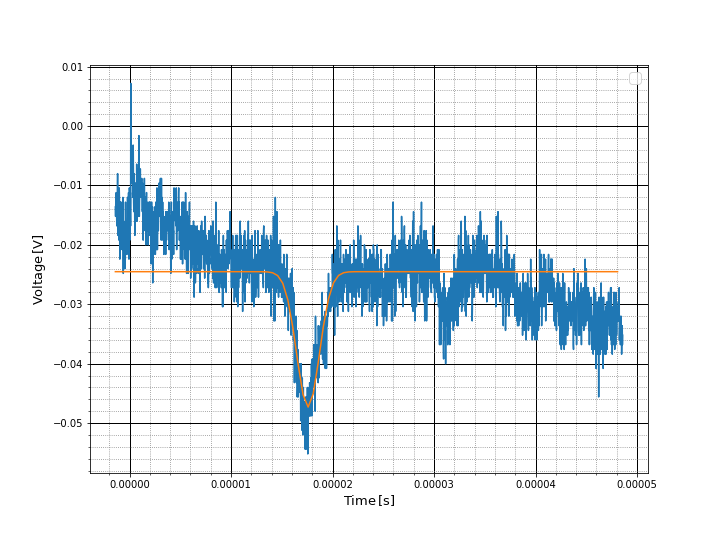
\includegraphics[scale=0.5]{Bild/S3}
	\centering
	\caption[Gaußfit an Messung bei Konst. Spannung 3]{Gaußfit an die Messungen der Elektronenwolken bei  einer Spannung von $48\,$V und einem Abstand zwischen Nadel und Lase von $8.6$\,mm.}
\end{figure}
\begin{figure}
	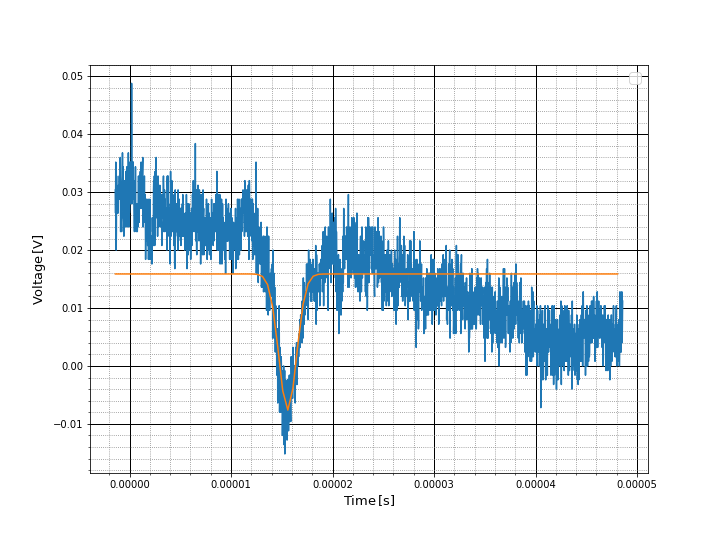
\includegraphics[scale=0.5]{Bild/S4}
	\centering
	\caption[Gaußfit an Messung bei Konst. Spannung 4]{Gaußfit an die Messungen der Elektronenwolken bei  einer Spannung von $48\,$V und einem Abstand zwischen Nadel und Lase von $7.6$\,mm.}
\end{figure}
\begin{figure}
	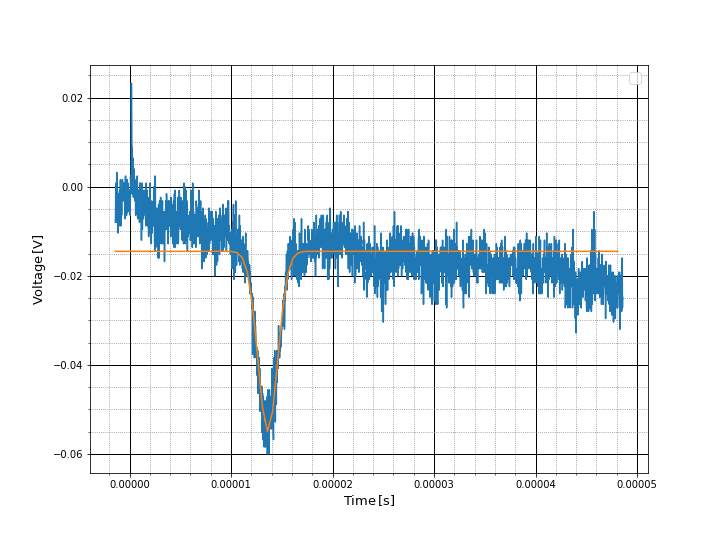
\includegraphics[scale=0.5]{Bild/S5}
	\centering
	\caption[Gaußfit an Messung bei Konst. Spannung 5]{Gaußfit an die Messungen der Elektronenwolken bei einer Spannung von $48\,$V und einem Abstand zwischen Nadel und Lase von $6.6$\,mm.}
\end{figure}
\begin{figure}
	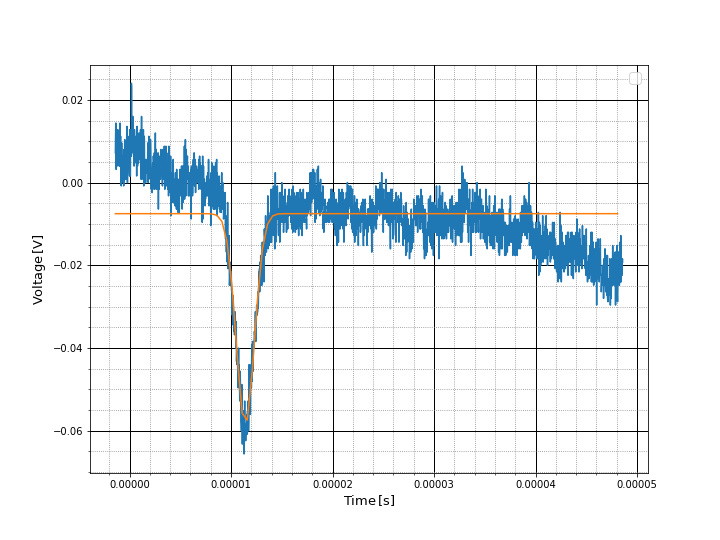
\includegraphics[scale=0.5]{Bild/S6}
	\centering
	\caption[Gaußfit an Messung bei Konst. Spannung 6]{Gaußfit an die Messungen der Elektronenwolken bei einer Spannung von $48\,$V und einem Abstand zwischen Nadel und Lase von $5.6$\,mm.}
\end{figure}
\begin{figure}
	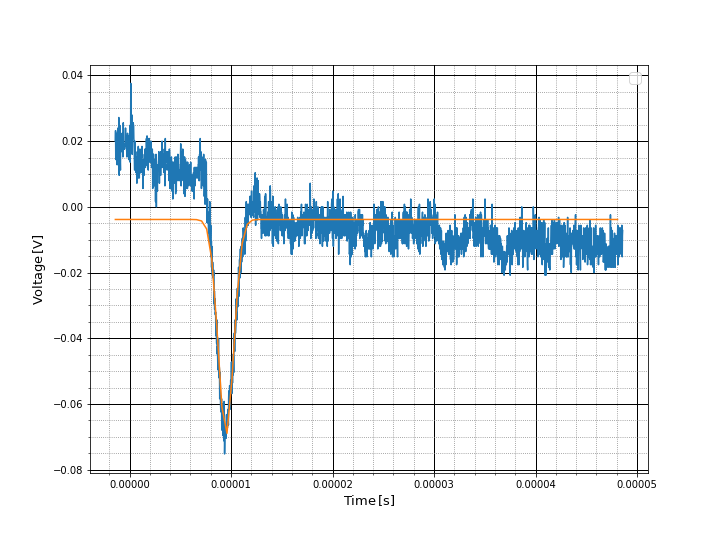
\includegraphics[scale=0.5]{Bild/S7}
	\centering
	\caption[Gaußfit an Messung bei Konst. Spannung 7]{Gaußfit an die Messungen der Elektronenwolken bei einer Spannung von $48\,$V und einem Abstand zwischen Nadel und Lase von $4.6$\,mm.}
\end{figure}
\begin{figure}
	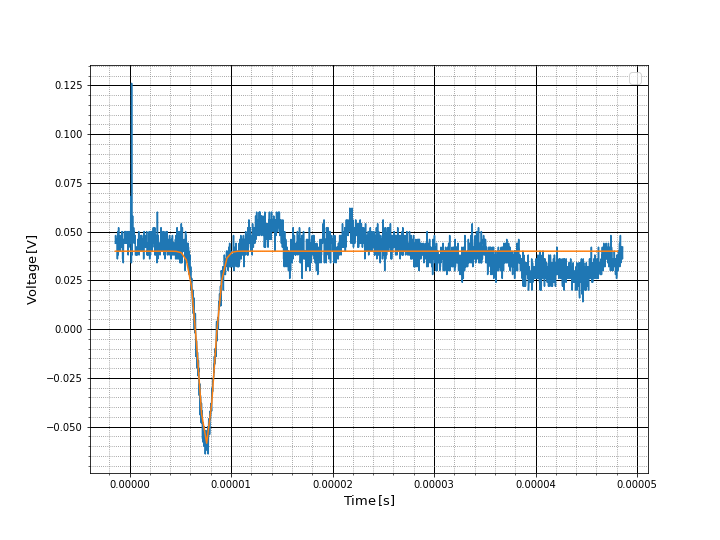
\includegraphics[scale=0.5]{Bild/S8}
	\centering
	\caption[Gaußfit an Messung bei Konst. Spannung 8]{Gaußfit an die Messungen der Elektronenwolken bei einer Spannung von $48\,$V und einem Abstand zwischen Nadel und Lase von $3.6$\,mm.}
\end{figure}

%Andere Messreihe

\begin{figure}
	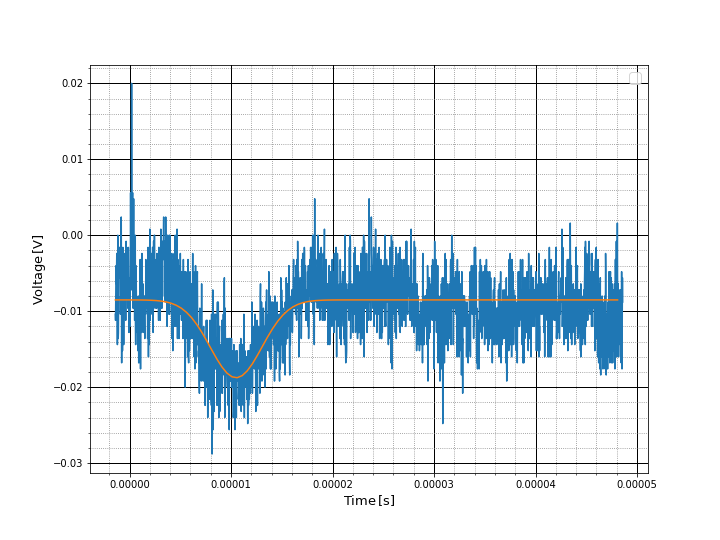
\includegraphics[scale=0.5]{Bild/A1}
	\centering
	\caption[Gaußfit an Messung bei Konst. Abstand]{Gaußfit an die Messungen der Elektronenwolken bei Konstantem Abstand von $3.6$\,mm und einer Spannung von $-13.2$\,V}
\end{figure}
\begin{figure}
	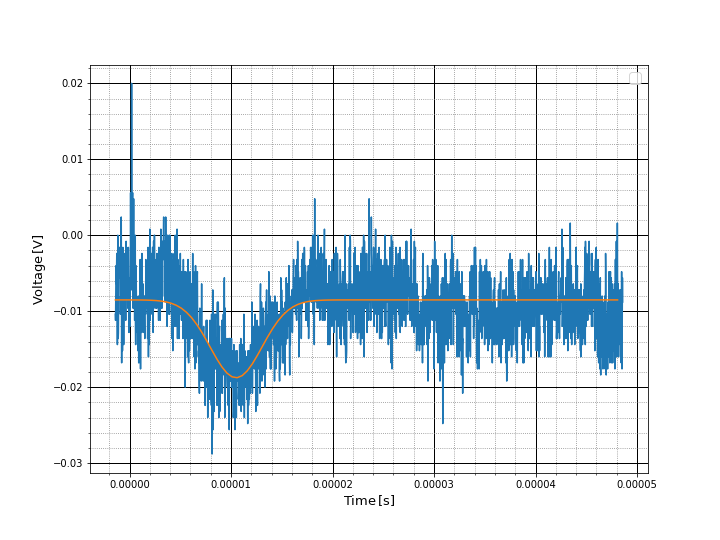
\includegraphics[scale=0.5]{Bild/A1}
	\centering
	\caption[Gaußfit an Messung bei Konst. Abstand]{Gaußfit an die Messungen der Elektronenwolken bei Konstantem Abstand von $3.6$\,mm und einer Spannung von $-15.2$\,V}
\end{figure}
\begin{figure}
	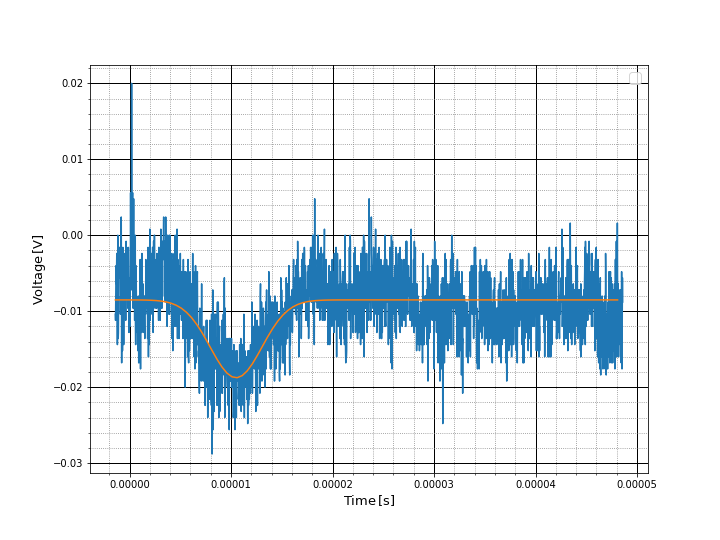
\includegraphics[scale=0.5]{Bild/A1}
	\centering
	\caption[Gaußfit an Messung bei Konst. Abstand]{Gaußfit an die Messungen der Elektronenwolken bei Konstantem Abstand von $3.6$\,mm und einer Spannung von $-18.4$\,V}
\end{figure}
\begin{figure}
	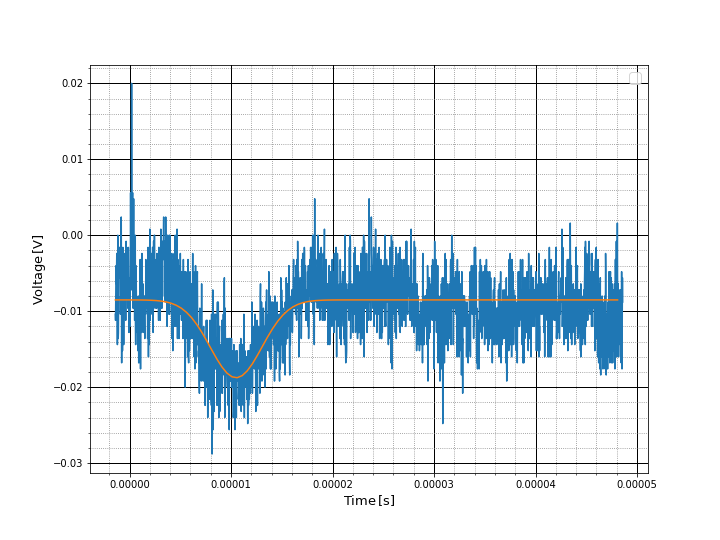
\includegraphics[scale=0.5]{Bild/A1}
	\centering
	\caption[Gaußfit an Messung bei Konst. Abstand]{Gaußfit an die Messungen der Elektronenwolken bei Konstantem Abstand von $3.6$\,mm und einer Spannung von $-20.4$\,V}
\end{figure}
\begin{figure}
	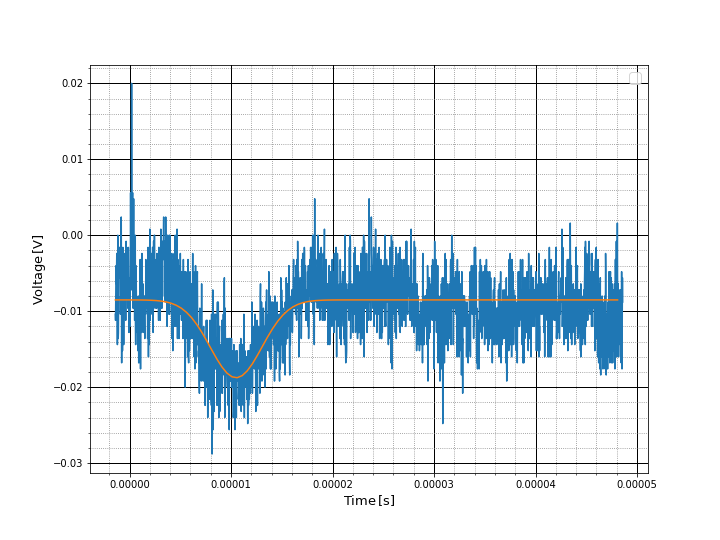
\includegraphics[scale=0.5]{Bild/A1}
	\centering
	\caption[Gaußfit an Messung bei Konst. Abstand]{Gaußfit an die Messungen der Elektronenwolken bei Konstantem Abstand von $3.6$\,mm und einer Spannung von $-22.4$\,V}
\end{figure}
\begin{figure}
	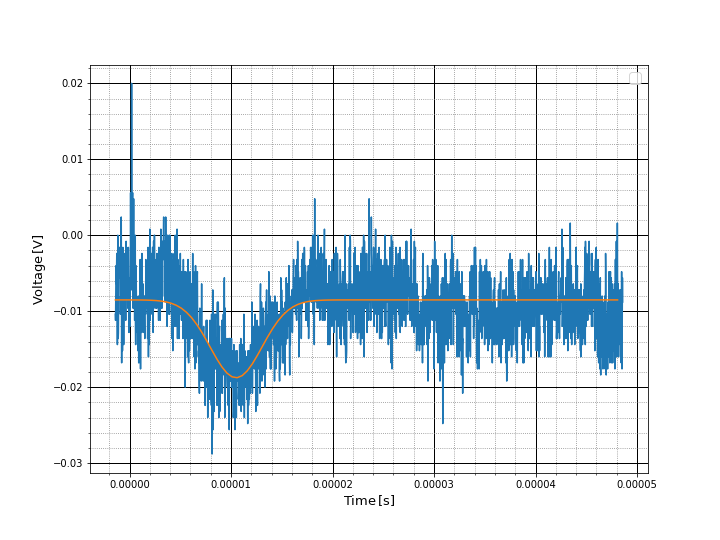
\includegraphics[scale=0.5]{Bild/A1}
	\centering
	\caption[Gaußfit an Messung bei Konst. Abstand]{Gaußfit an die Messungen der Elektronenwolken bei Konstantem Abstand von $3.6$\,mm und einer Spannung von $-24.4$\,V}
\end{figure}
\begin{figure}
	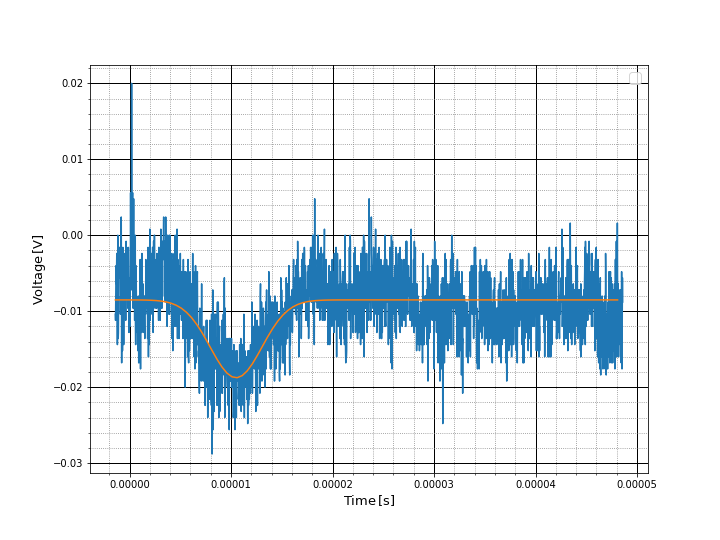
\includegraphics[scale=0.5]{Bild/A1}
	\centering
	\caption[Gaußfit an Messung bei Konst. Abstand]{Gaußfit an die Messungen der Elektronenwolken bei Konstantem Abstand von $3.6$\,mm und einer Spannung von $-28.0$\,V}
\end{figure}
\begin{figure}
	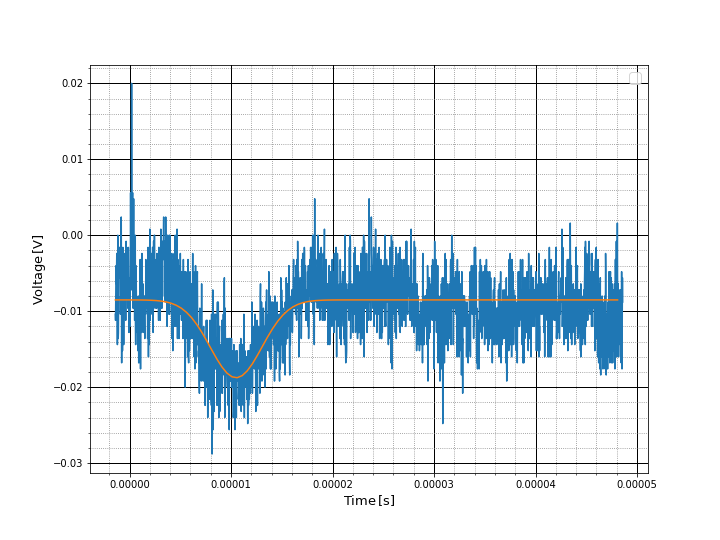
\includegraphics[scale=0.5]{Bild/A1}
	\centering
	\caption[Gaußfit an Messung bei Konst. Abstand]{Gaußfit an die Messungen der Elektronenwolken bei Konstantem Abstand von $3.6$\,mm und einer Spannung von $-32.0$\,V}
\end{figure}
\begin{figure}
	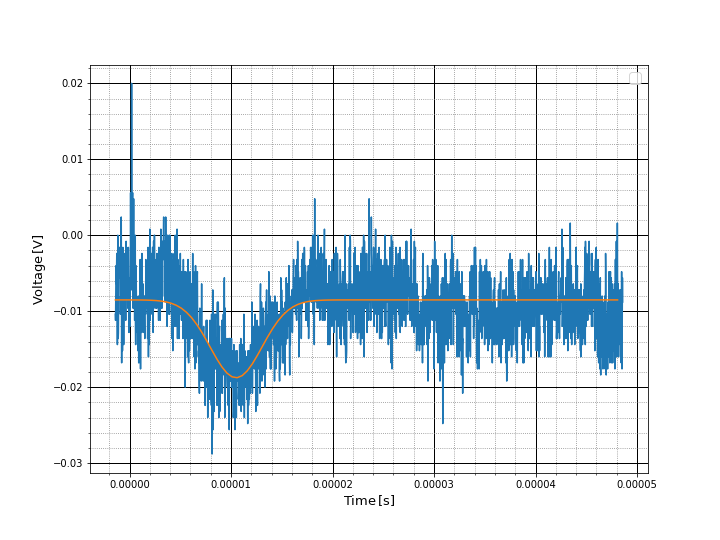
\includegraphics[scale=0.5]{Bild/A1}
	\centering
	\caption[Gaußfit an Messung bei Konst. Abstand]{Gaußfit an die Messungen der Elektronenwolken bei Konstantem Abstand von $3.6$\,mm und einer Spannung von $-36.0$\,V}
\end{figure}
\begin{figure}
	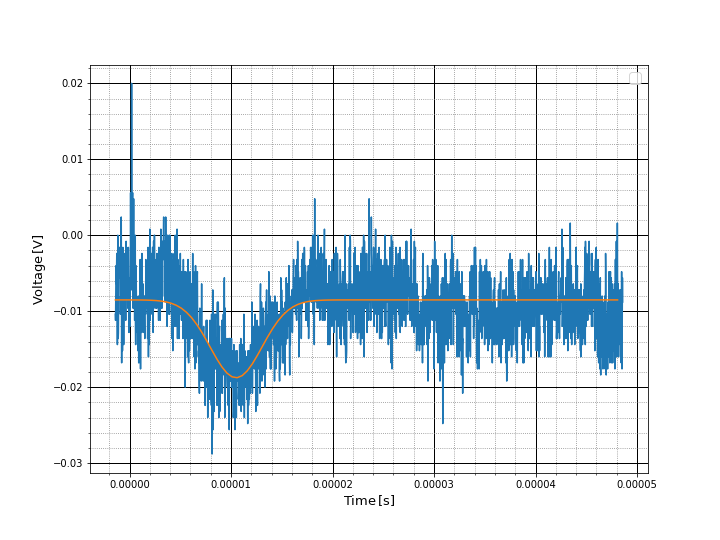
\includegraphics[scale=0.5]{Bild/A1}
	\centering
	\caption[Gaußfit an Messung bei Konst. Abstand]{Gaußfit an die Messungen der Elektronenwolken bei Konstantem Abstand von $3.6$\,mm und einer Spannung von $-40.0$\,V}
\end{figure}
\begin{figure}
	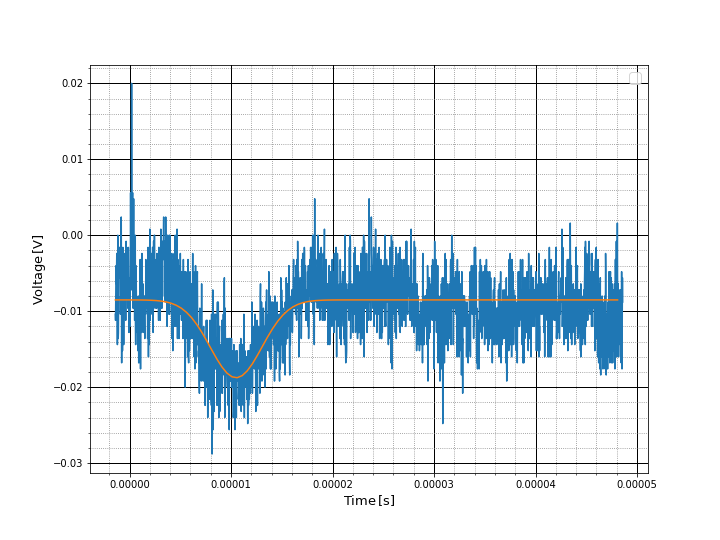
\includegraphics[scale=0.5]{Bild/A1}
	\centering
	\caption[Gaußfit an Messung bei Konst. Abstand]{Gaußfit an die Messungen der Elektronenwolken bei Konstantem Abstand von $3.6$\,mm und einer Spannung von $-44.0$\,V}
\end{figure}
\begin{figure}
	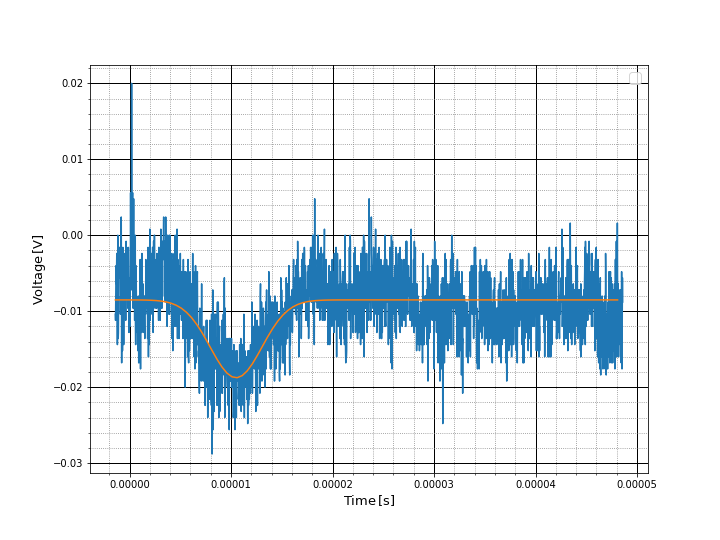
\includegraphics[scale=0.5]{Bild/A1}
	\centering
	\caption[Gaußfit an Messung bei Konst. Abstand]{Gaußfit an die Messungen der Elektronenwolken bei Konstantem Abstand von $3.6$\,mm und einer Spannung von $-46.0$\,V}
\end{figure}
\begin{figure}
	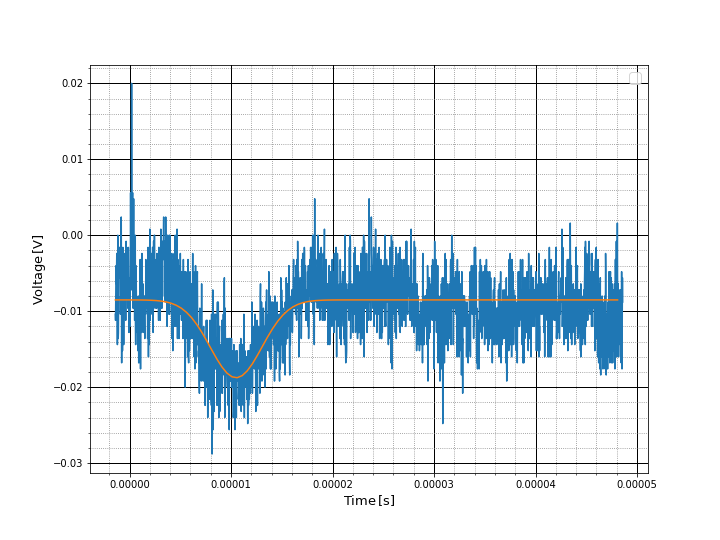
\includegraphics[scale=0.5]{Bild/A1}
	\centering
	\caption[Gaußfit an Messung bei Konst. Abstand]{Gaußfit an die Messungen der Elektronenwolken bei Konstantem Abstand von $3.6$\,mm und einer Spannung von $-48.0$\,V}
\end{figure}

%Lange Messungen

\begin{figure}[ht]
	\includegraphics[scale=0.5]{Bild/ASg}
	\centering
	\caption{Gesamtes Spektrum von Americium mit Silizium aufgenommen.}
\end{figure}
\begin{figure}[ht]
	\includegraphics[scale=0.5]{Bild/ACg}
	\centering
	\caption{Gesamtes Spektrum von Americium mit CdTe aufgenommen.}
\end{figure}
\begin{figure}[ht]
	\includegraphics[scale=0.5]{Bild/CSg}
	\centering
	\caption{Gesamtes Spektrum von Cobalt mit Silizium aufgenommen.}
\end{figure}
\begin{figure}[ht]
	\includegraphics[scale=0.5]{Bild/CCg}
	\centering
	\caption{Gesamtes Spektrum von Cobalt mit CdTe aufgenommen.}
\end{figure}
\subsection{Laborbuch}
%\includepdf[pages=-,scale=0.8]{Bilder/anhang/Halbleiter.pdf}
\end{document}